\chapter{Overview} \label{ch:OverView}
\chapterquote{Always be in readiness to serve the cause of humanity. Select the kind of work you are qualified to do by your individual aptitude and abilities. And whatever service you can render must faithfully be carried out.}{Meher Baba}


\graphicspath{{Chapters/Overview/Figures/}}
\lstinputpath{Codes-VHDL/Chapter-Overview/VHDLCodes/} %path is defined in mypreamble


%\section{Introduction}
In this chapter, UART communication is discussed for NIOS design. Values of Sin(x) is generated using NIOS and the data is  received by computer using UART cable. Since, onchip memory is smaller for storing these values, therefore external memory i.e. SDRAM is used. Further, the received data is stored in a file using `Tera Term' software; finally live-plotting of data is performed using Python.  

In this chapter, we will learn following topics, 
\begin{enumerate}
	\item UART interface,
	\item Receiving the data on computer using UART communication,
	\item SDRAM interface,
	\item Saving data generated by NIOS desgin to a file using `Tera Term',
	\item Updating a existing QSys design and corresponding VHDL and NIOS design,
	\item Live-plotting of data using Python. 
\end{enumerate}

\section{UART interface}
First, create a empty project with name `UartComm' (see Section \ref{sec:new_project}). Next, open the QSys from Tools$\rightarrow$Qsys. Add `Nios Processor', `On-chip RAM (with 20k total-memory-size), `JTAG UART' and `UART (RS-232 Serial Port)' (\textbf{all with default settings}). Note that, Baud rate for UART is set to `115200' (see Fig. \ref{fig:uart_settings}), which will be used while getting the data on computer. Lastly, connect these items as shown in Fig. \ref{fig:uart_qsys_conn}; save it as `Uart\_Qsys.qsys' and finally generate the Qsys system and close the Qsys. Please see Section \ref{sec:CreateGenerateQsys}, if you have problem in generating the QSys system.

\begin{figure}[!h]
	\centering
	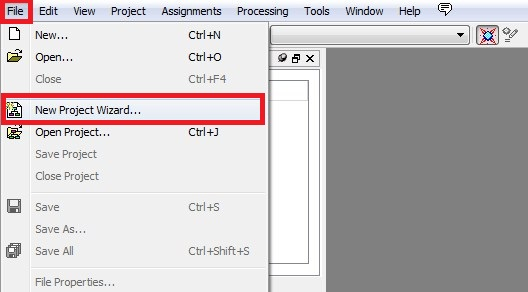
\includegraphics[scale=0.7]{1}
	\caption{UART settings}
	\label{fig:uart_settings}
\end{figure}
 
\begin{figure}[!h]
	\centering
	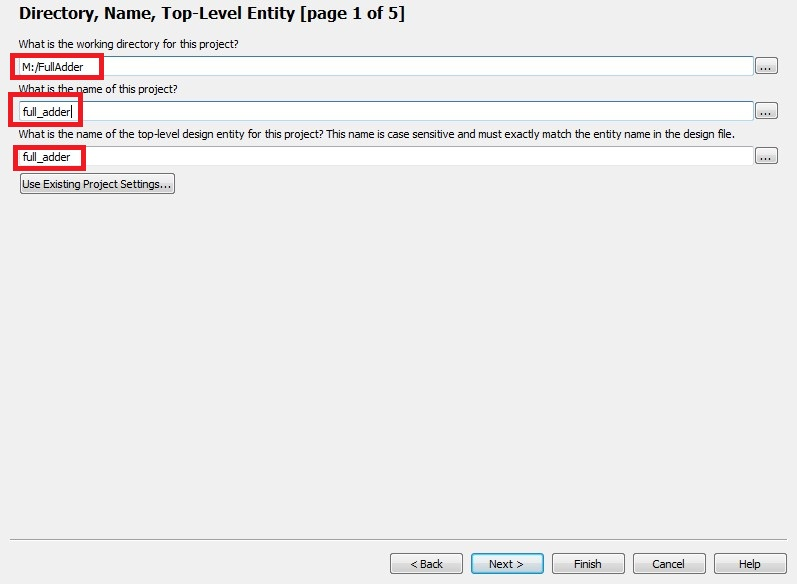
\includegraphics[scale=0.65]{2}
	\caption{Qsys connections}
	\label{fig:uart_qsys_conn}
\end{figure}

Now, add the file `Uart\_Qsys.qip' to the VHDL project. Next, create a new `Block diagram (.bdf) file and import the Qsys design to it and assign correct pin numbers to it, as shown in Fig. \ref{fig:uart_top}. Save it as `Uart\_top.bdf' and set it as `top  level entity'. Lastly, import the pin assignment file and compile the design. Finally, load the design on FPGA board. 

\begin{figure}[!h]
	\centering
	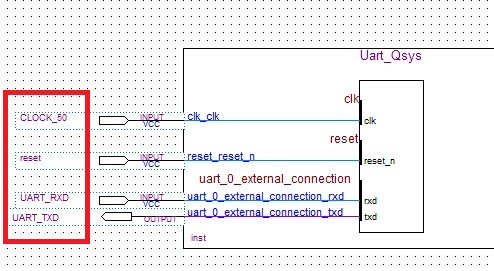
\includegraphics[scale=0.65]{3}
	\caption{Top level entity `Uart\_top.bdf'}
	\label{fig:uart_top}
\end{figure}

\section{NIOS design}
In Chapter \ref{ch:NiosOverview}, we created the `BSP' and `application' file separately for NIOS design. In this chapter, we will use the template provided with NIOS to create the design. For this, open the NIOS software and go to `Files$\rightarrow$New$\rightarrow$NIOS II Application and BSP from Template'. Next, Select the `UART\_Qsys.sopcinfo' file and `Hello World' template and provide the desired name to project e.g. UART\_comm\_app, as shown in Fig , and click `next'. In this window, enter the desired name for BSP file in the `Project name' column e.g. `UART\_comm\_bsp'; and click on Finish.  

\begin{figure}[!h]
	\centering
	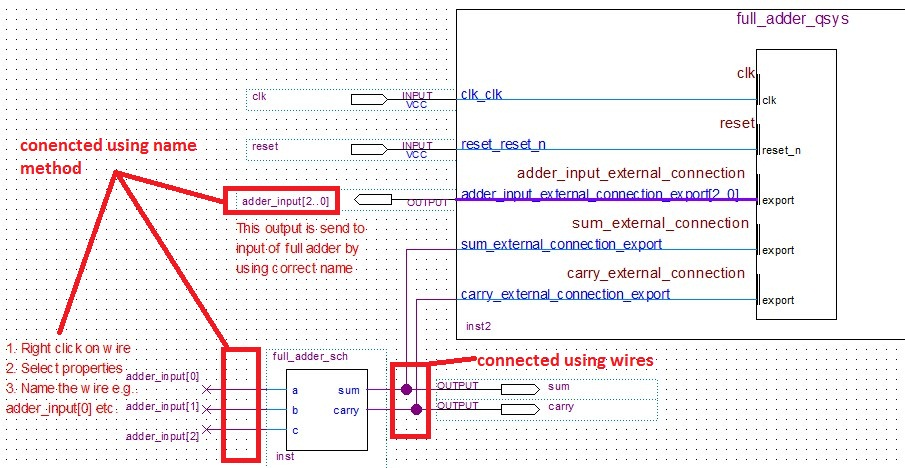
\includegraphics[scale=0.65]{4}
	\caption{Create NIOS project from template}
	\label{fig:nios_name_uart}
\end{figure}

\section{Communication through UART}
To received the data on computer, we need some software like Putty or Tera Term. In this tutorial, we are using `Tera Term software, which can be downloaded freely. Also, we need to change the UART communication settings; so that, we can get messages through UART interface (instead of JTAG-UART)  as shown next. 

Right click on `UART\_comm\_bsp' and go to `NIOS II$\rightarrow$BSP editor'; and select UART\_115200 for various communication as shown in Fig \ref{fig:nios_uart_settings}; and finally click on generate and then click on exit. Now, all the 	`printf' statements will be send to computer via UART port (instead of Jtag-uart). We can change it to JTAG-UART again, by changing UART\_115200 to JTAG-UART again. Note that, when we modify the BSP using BSP-editor, then we need to generate the system again.

\begin{figure}[!h]
	\centering
	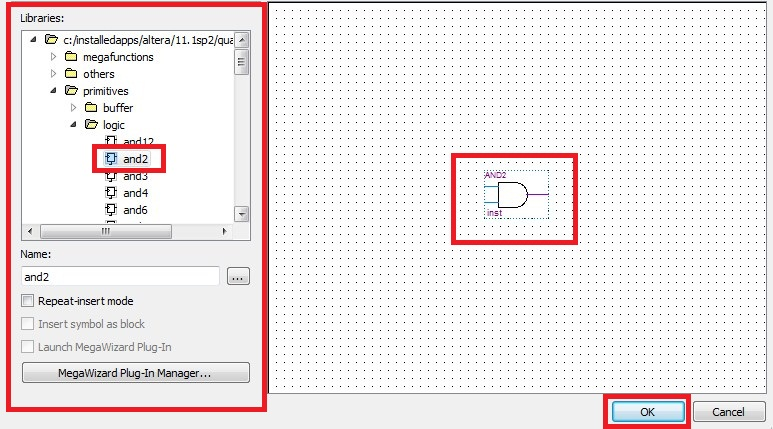
\includegraphics[scale=0.65]{5}
	\caption{UART communication settings in NIOS}
	\label{fig:nios_uart_settings}
\end{figure}

Now, open the Tera Term and select the `Serial' as shown in Fig. \ref{fig:teraTerm}. Then go to `Setup$\rightarrow$Serial Port...' and select the correct baud rate i.e. 115200 and click OK, as shown in Fig. \ref{fig:baudRateteraTerm}. 

\begin{figure}[!h]
	\centering
	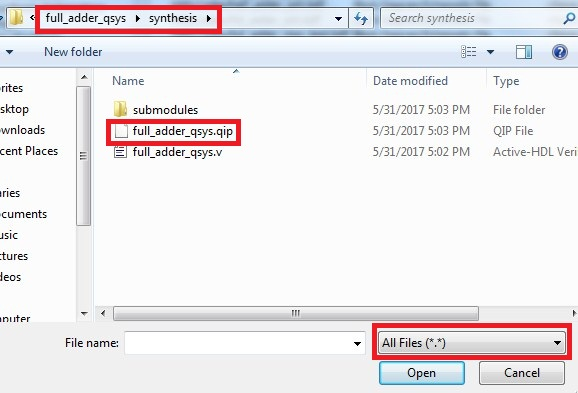
\includegraphics[scale=0.65]{6}
	\caption{Serial communication in Tera Term}
	\label{fig:teraTerm}
\end{figure}

\begin{figure}[!h]
	\centering
	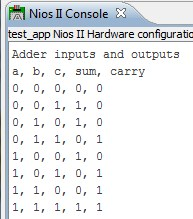
\includegraphics[scale=0.65]{7}
	\caption{Select correct baud rate}
	\label{fig:baudRateteraTerm}
\end{figure}

Finally, right click on `UART\_comm\_app' in NIOS and go to `Run As$\rightarrow$3 NIOS 2 Hardware'. Now, we can see the output on the Tera Term terminal, as shown in Fig. \ref{fig:helloTera}. 

\begin{figure}[!h]
	\centering
	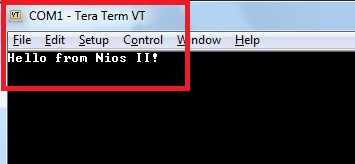
\includegraphics[scale=0.65]{8}
	\caption{`Hello from NIOS II!' on Tera Term}
	\label{fig:helloTera}
\end{figure}

\section{SDRAM Interface}
Our next aim is to generate the Sine waves using NIOS and then plot the waveforms using python. If we write the C-code in current design, then our system will report the memory issue as onchip memory is too small; therefore we need to use external memory. In this section, first, we will update the Qsys design with SDRAM interface, then we will update the Quartus design and finally add the C-code to generate the Sine waves. 

\subsection{Modify QSys}
First, Open the UART\_Qsys.qsys file in QSys software. Now, add SDRAM controller with default settings,  as shown in Fig. \ref{fig:sdram_con}. Next, connect all the ports of SDRMA as shown in Fig. \ref{fig:sdram_connections}. Then, double click the `nios2\_qsys\_0' and select `SDRAM' as reset and exception vector memory, as shown in Fig. \ref{fig:sdram_vector_memory}. 

\begin{figure}[!h]
	\centering
	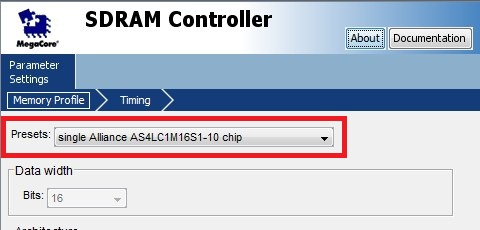
\includegraphics[scale=0.6]{9}
	\caption{SDRAM controller}
	\label{fig:sdram_con}
\end{figure}


\begin{figure}[!h]
	\centering
	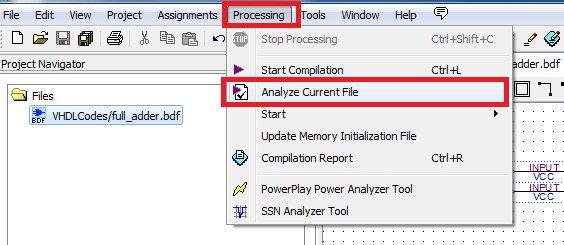
\includegraphics[scale=0.6]{10}
	\caption{SDRAM connections}
	\label{fig:sdram_connections}
\end{figure}


\begin{figure}[!h]
	\centering
	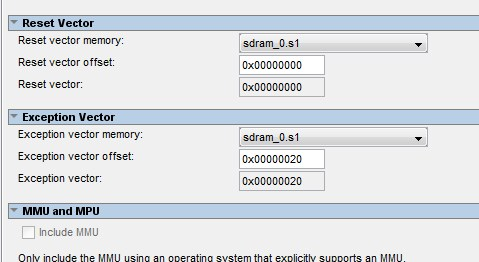
\includegraphics[scale=0.6]{11}
	\caption{Select SDRAM as vector memories}
	\label{fig:sdram_vector_memory}
\end{figure}


Next, we will add `Switches' to control the amplitude of the sine waves. For this add the PIO device of `8 bit with type input', and rename it as `switch', as shown in Fig. \ref{fig:switchForAmplitude} . Finally, go to System$\rightarrow$Assign base addresses, and generate the system. 

\begin{figure}[!h]
	\centering
	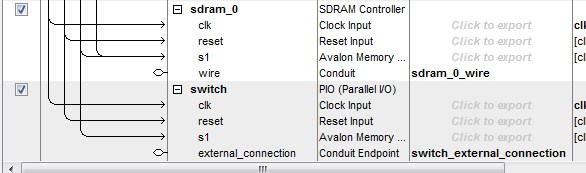
\includegraphics[scale=0.65]{12}
	\caption{Add switches for controlling the amplitude of sine waves}
	\label{fig:switchForAmplitude}
\end{figure}


\subsection{Modify Top level Quartus design}
Now, open the `Uart\_top.bdf' file in Quartus. Right click on the `Uart\_Qsys' block and select `Update symbol or block'; then select the option `Selected symbol(s) or block(s)' and press OK. It will display all the ports for `SDRAM' and switches. Next, we need to assign the correct `pin names' to these ports, as shown in Fig. \ref{fig:SDRAM_Pinassg}.  

\begin{figure}[!h]
	\centering
	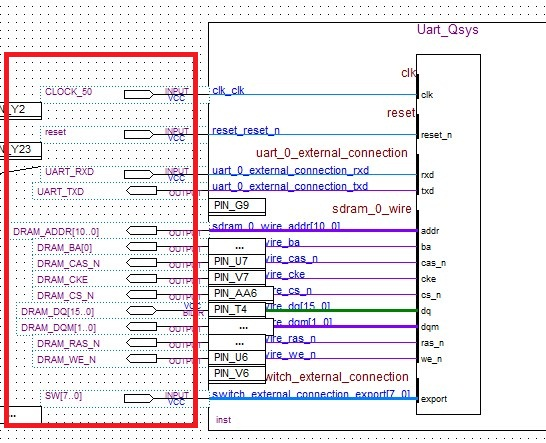
\includegraphics[scale=0.65]{13}
	\caption{Assigning Pins to SDRAM and Switches}
	\label{fig:SDRAM_Pinassg}
\end{figure}

Note that, there should be `-3 ns clock delay' for SDRAM as compare to FPGA clock, therefore we need to add the clock with `-3 ns delay'. For this, double click on the Uart\_top.bdf (anywhere in the file), and select `MegaWizard Plug-In Manager'. Then select `Create a new custom megafunction variation' in the popped-up window and click next. Now, select \textbf{ALTPLL} from \textbf{IO} in \textbf{Installed Plug-Ins} option, as shown in Fig. \ref{fig:dram_clock_altpll}, and click next. Then, follow the figures from Fig. \ref{fig:altpllCreation1} to Fig. \ref{fig:altpllCreation6} to add the ALTPLL to current design i.e. `Uart\_top.bdf'. Finally, connect the ports of this design as shown in Fig. \ref{fig:altpllCreation7}. Note that, in these connections, output of ATLPLL design is connected to `DRAM\_CLK', which is clock-port for DRAM. Lastly, compile and load the design on FPGA board. 

\begin{figure}[!h]
	\centering
	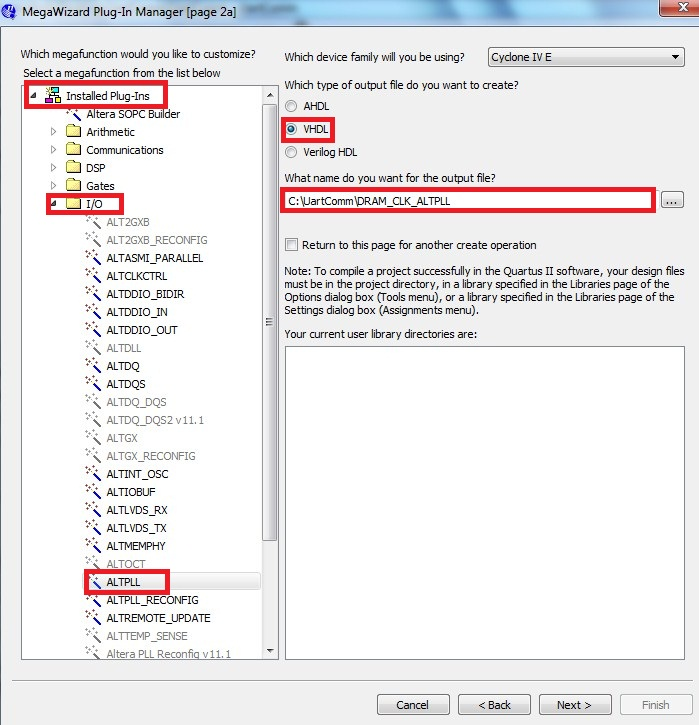
\includegraphics[scale=0.4]{14}
	\caption{ALTPLL generation}
	\label{fig:dram_clock_altpll}
\end{figure}

\begin{figure}[!h]
	\centering
	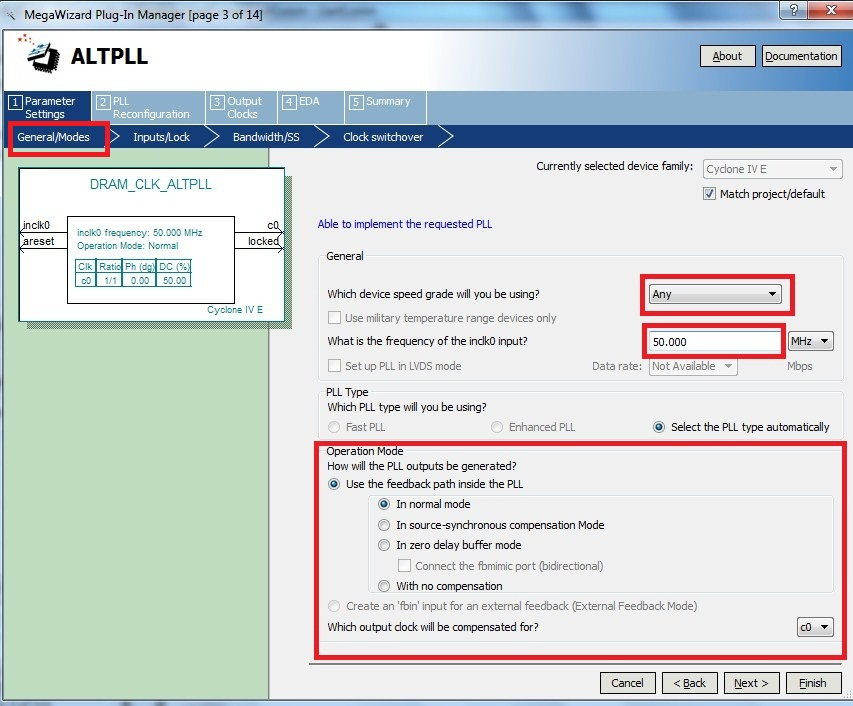
\includegraphics[scale=0.4]{15}
	\caption{ALTPLL creation, step 1}
	\label{fig:altpllCreation1}
\end{figure}

\begin{figure}[!h]
	\centering
	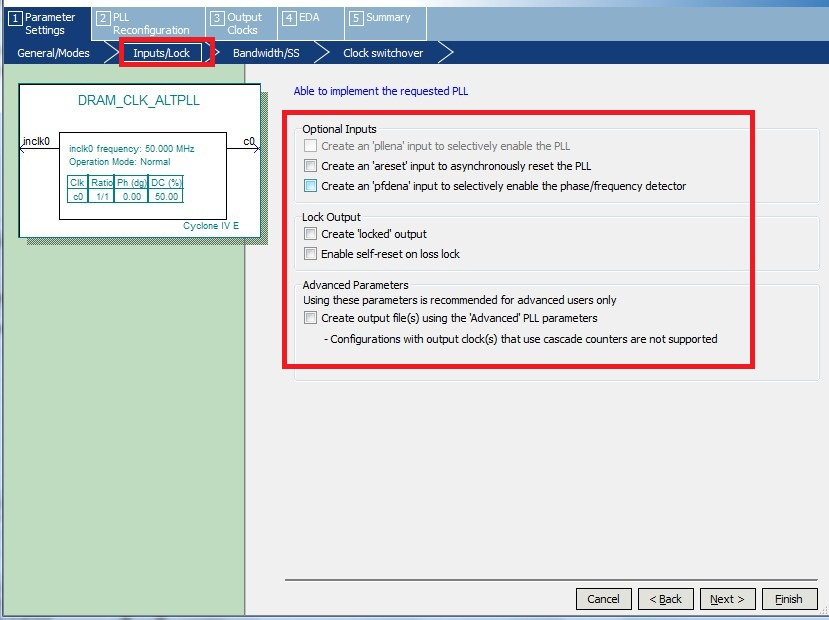
\includegraphics[scale=0.5]{16}
	\caption{ALTPLL creation, step 2}
	\label{fig:altpllCreation2}
\end{figure}

\begin{figure}[!h]
	\centering
	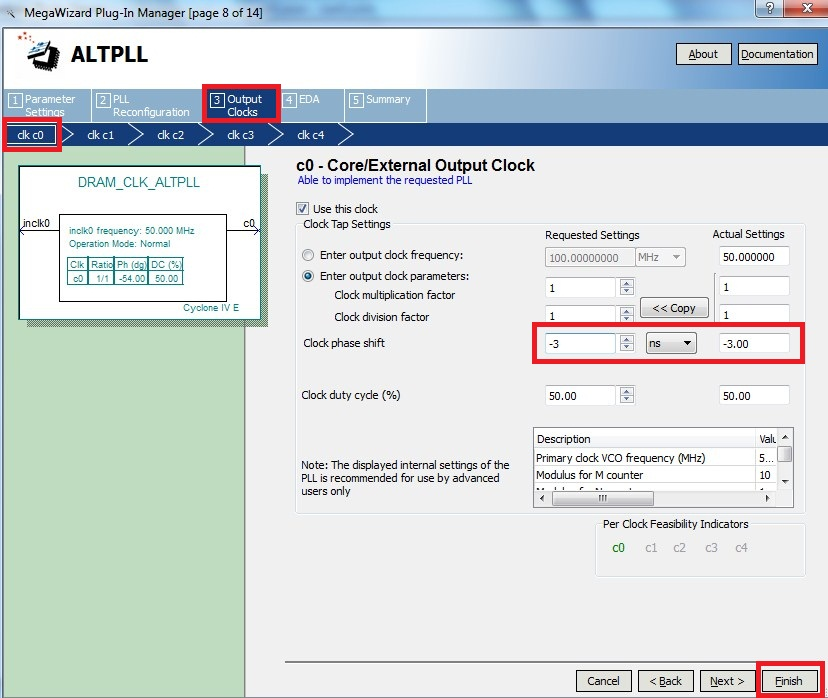
\includegraphics[scale=0.4]{17}
	\caption{ALTPLL creation, step 3}
	\label{fig:altpllCreation3}
\end{figure}

\begin{figure}[!h]
	\centering
	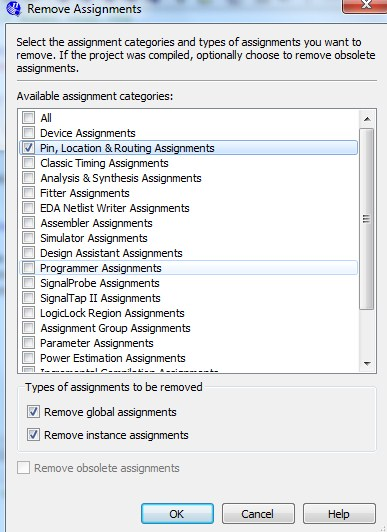
\includegraphics[scale=0.4]{18}
	\caption{ALTPLL creation, step 4}
	\label{fig:altpllCreation4}
\end{figure}

\begin{figure}[!h]
	\centering
	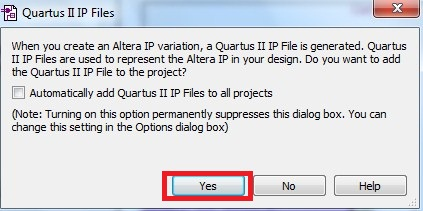
\includegraphics[scale=0.5]{19}
	\caption{ALTPLL creation, step 5}
	\label{fig:altpllCreation5}
\end{figure}

\begin{figure}[!h]
	\centering
	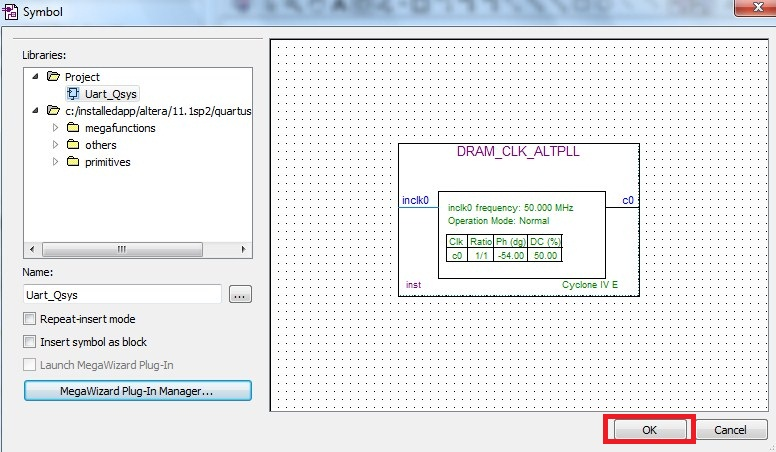
\includegraphics[scale=0.5]{20}
	\caption{ALTPLL creation, step 6}
	\label{fig:altpllCreation6}
\end{figure}

\begin{figure}[!h]
	\centering
	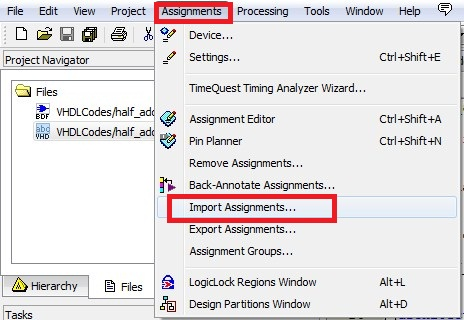
\includegraphics[scale=0.6]{21}
	\caption{Connect ALTPLL design with existing design}
	\label{fig:altpllCreation7}
\end{figure}

\subsection{Updating NIOS design}
Since, we have udpated the QSys design, therefore the corresponding .sopcinfo file is also updated. Further, BSP files depends on the .sopcinfo file, therefore we need to update the BSP as well. For this, right click on `Uart\_comm\_bsp' and go to `NIOS II$\rightarrow$BSP Editor; and update the BSP as shown in Fig. \ref{fig:updateBSPDRAM} and click on `generate' and then click `exit'. Note that, `enable' options are unchecked now, because we are using External memory, which is quite bigger than onchip-memory, so we do not need `small' size options. 

\begin{figure}[!h]
	\centering
	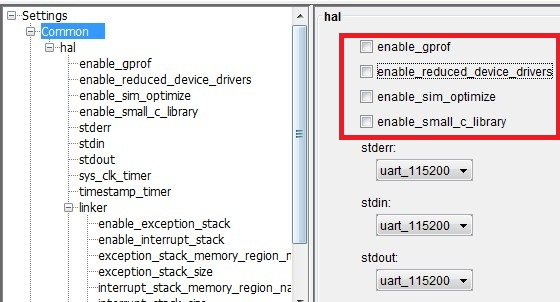
\includegraphics[scale=0.65]{22}
	\caption{Update BSP for new Qsys design}
	\label{fig:updateBSPDRAM}
\end{figure}

Now, update the `hello\_world.c' file as shown in Listing \ref{c:uart_sine_wave}. 

\lstinputlisting[
caption    = {Sin and Cos wave generation},
language = C,
label      = {c:uart_sine_wave}
]{CppCodes/hello_world.c}

In Tera Term, we can save the received values in text file as well. Next, go Files$\rightarrow$Log and select the filename at desired location to save the data e.g. `sineData.txt'. 

Finally, right click on `UART\_comm\_app' in NIOS and go to `Run As$\rightarrow$3 NIOS 2 Hardware'. Now, we can see the decimal values on the screen. If all the switches are at `0' position, then values will be `0.000' as amplitude is zero. Further, we can use any combination of 8 Switches to increase the amplitude of the sine and cosine waves. Also, result will be stored in the  `sineData.txt' file. Content of this file is shown in Fig. \ref{fig:contentLogFile}


\begin{figure}[!h]
	\centering
	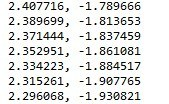
\includegraphics[scale=0.8]{23}
	\caption{Content of `sineData.txt' file}
	\label{fig:contentLogFile}
\end{figure}

\section{Live plotting the data}
In the previous section, we store the sine and cosine wave data on the `sineData.txt' using UART communication. Now, our last task is to plot this data continuously, so that it look line animation. For this save the Listing \ref{pythhon:plotLogData}, in the location where `sineData.txt' is saved. Now, open the command prompt and go to the location of python file. Finally, type \textbf{`python main.py'} and press enter. This will start plotting the waveform continuously based on the data received and stored on the `sineData.txt' file. The corresponding plots are shown in Fig. \ref{fig:plotLogFile}.

\lstinputlisting[
caption    = {Code for live plotting of logged data},
language = Python,
label      = {pythhon:plotLogData}
]{PythonCodes/main.py}

\begin{figure}[!h]
	\centering
	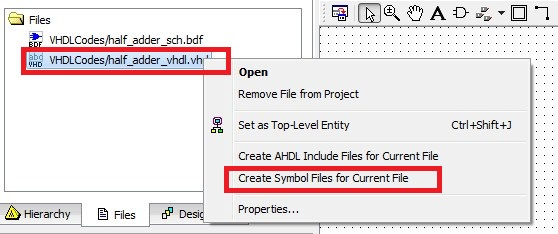
\includegraphics[scale=0.5]{24}
	\caption{Plot of `sineData.txt' file}
	\label{fig:plotLogFile}
\end{figure}


\section{Conclusion}
In this chapter, first we display the `Hello' message using UART and Tera Term. Then, SDRAM is included in the design and correspondingly all the other designs are updated i.e. Quartus and NIOS. Then, the data is stored in the text file and finally it is plotted with the help of Python programming language. 
%\section{Entity and Architecture}
In this section, we discuss `entity declaration' and `architecture body' along with three different ways of modeling i.e. `data flow', 'structural' and `behavioral' modeling. In practice, these three styles are mixed together to model a digital circuit.  

\subsection{Entity declaration}
In Fig. \ref{fig:andEx}, a simple `and' gate is shown; which is generated by Listing \ref{vhdl:andEx}. Listing \ref{vhdl:andEx} is included to understand the meaning of `entity declaration' and `architecture body'. Also in VHDL, `$--$' is used for comments; please read comments as well to understand the codes.

The entity declaration (lines 6-11) contains all the name of the input and outputs ports as shown in Listing \ref{vhdl:andEx}. Here, the design has two input ports i.e. $x$ and $y$ and one output port i.e. $z$, which are defined inside the `port' block in line 7. Name of the entity `andEx' is defined in line 6. Lastly, we need to import libraries to the listing which contains various functions e.g. library `IEEE' (line 3) contains the package `std\_logic\_1164' (line 4), in which `std\_logic' is defined. `std\_logic' is used in line 8 and 9, to define the 1-bit input and output data-types. Lastly, entity block is closed with `end' keyword in line 11. All these terms, i.e. IEEE library and packages along with data-types, are discussed in detail in Chapter \ref{ch:Datatypes}.  

\begin{figure}
	\centering
	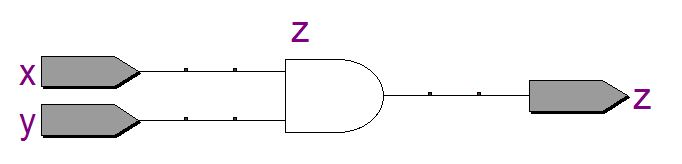
\includegraphics[scale=0.5]{andEx}
	\caption{Circuit generated by Listing \ref{vhdl:andEx}}
	\label{fig:andEx}
\end{figure}

\lstinputlisting[
language = Vhdl,
caption    = {`and' gate example, design: \ref{fig:andEx}},
label      = {vhdl:andEx}
]{andEx.vhd}

\subsection{Architecture body}
Actual behavior of the design is defined in  the `architecture body'. In Listing \ref{vhdl:andEx}, `and' gate is implemented with `x' and `y' as input, and `z' as output. This behavior is defined in line 15. In line 13, the name of the architecture is defined as `arch' and then name of the entity is given i.e. `andEx'. Complete logic is defined between `begin' and `end' statements i.e. line 14 and 16. Further, we can define intermediate signals of the design (i.e. apart from ports) between line 13-14 as shown in next sections. Next section contains more details about architecture body along with different modeling styles. 

\section{Modeling styles}
In VHDL, the architecture can be defined in four ways as shown in this section. Two bit comparator is designed with different styles; which generates the output `1' if the numbers are equal, otherwise output is set to `0'.   

\subsection{Dataflow modeling}
In this modeling style, the relation between input and outputs are defined using signal assignments. In the other words, we do not define the structure of the design explicitly; we only define the relationships between the signals; and structure is implicitly created during synthesis process. Listing \ref{vhdl:andEx} is the example of dataflow design, where relationship between inputs and output are given in line 15. 

\begin{table}
	\centering
	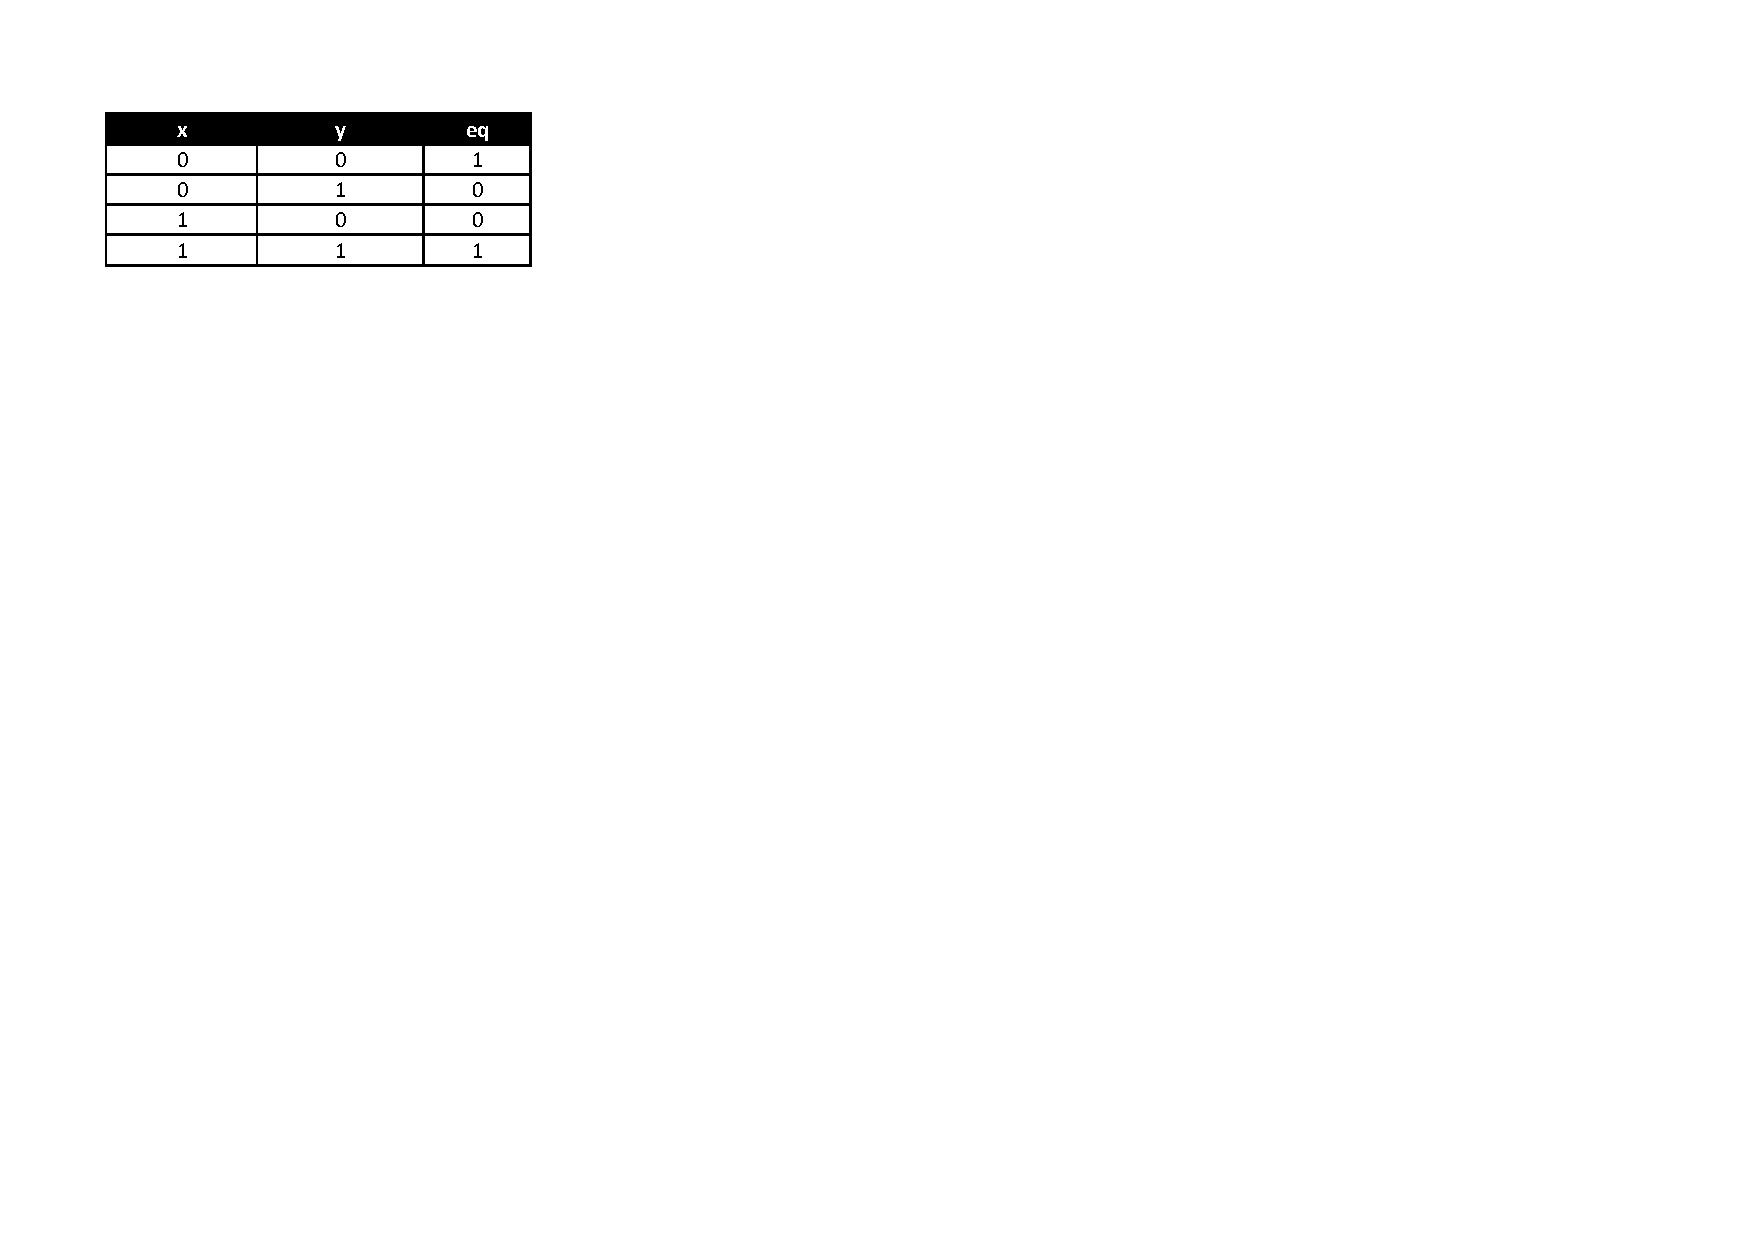
\includegraphics[scale=0.7]{TableComparator1Bit}
	\caption{1 bit comparator, Listing \ref{vhdl:comparator1Bit}}
	\label{tbl:comparator1Bit}
\end{table}

\begin{table}
	\centering
	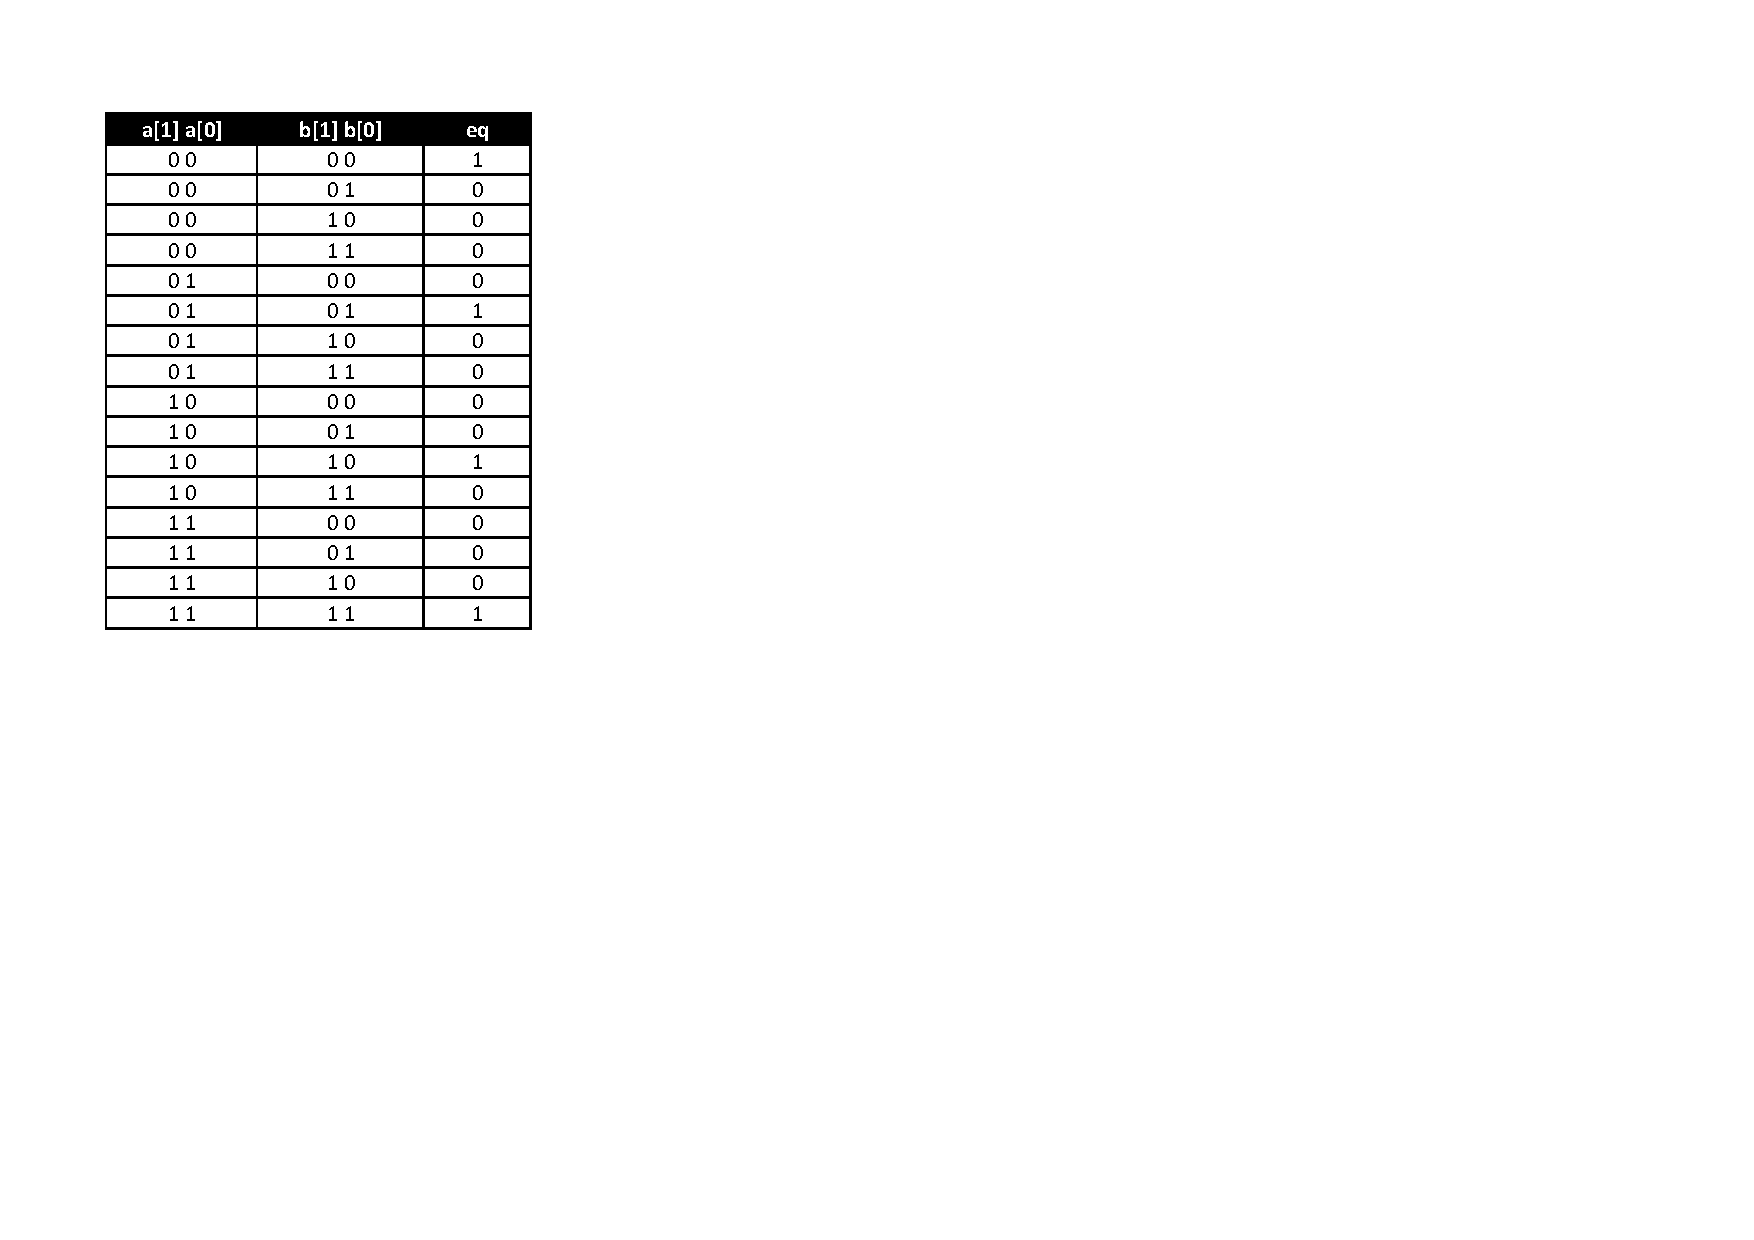
\includegraphics[scale=0.7]{TableComparator2Bit}
	\caption{2 bit comparator, Listing \ref{vhdl:comparator2Bit}}
	\label{tbl:comparator2Bit}
\end{table}

In this section, two more examples of dataflow modeling are shown i.e. `1 bit' and `2 bit' comparators; which are used to demonstrate the differences between various modeling styles in the tutorial. Table \ref{tbl:comparator1Bit} and \ref{tbl:comparator2Bit} show the truth tables of `1 bit' and `2 bit' comparators.  As the name suggests, the comparator compare the two values and sets the output `eq' to 1, when both the input values are equal; otherwise `eq' is set to zero. The corresponding boolean expressions are shown below, 

For 1 bit comparator: 
\begin{equation}
	eq = x' y' + x y
	\label{eq:1bitComparator}
\end{equation} 

For 2 bit comparator: 
\begin{equation}
eq = a'[1]a'[0]b'[1]b'[0] + a'[1]a[0]b'[1]b[0] + a[1]a'[0]b[1]b'[0] + a[1]a[0]b[1]b[0]
	\label{eq:2bitComparator}
\end{equation} 
Above two expressions are implemented using VHDL in Listing \ref{vhdl:comparator1Bit} and \ref{vhdl:comparator2Bit}, which are explained below.

\begin{explanation}[Listing \ref{vhdl:comparator1Bit}: 1 bit comparator]
	Listing \ref{vhdl:comparator1Bit} implements the 1 bit comparator based on equation \ref{eq:1bitComparator}. Two intermediate signals are defined between `architecture declaration' and `begin' statement (known as declaration section) as shown in line 14. These two signals ($s0$ and $s1$) are defined to store the values of $x'y'$ and $xy$ respectively. Values to these signals are assigned at line 16 and 17. Finally equation \ref{eq:1bitComparator} performs `or' operation on these two signals, which is done at line 19. When we compile this code using `Quartus software', it implements the code into hardware design as shown in Fig. \ref{fig:comparator1Bit}.
	
	The compilation process to generate the design is shown in Appendix \ref{QuartusModelsim}. Also, we can check the input-output relationships of this design using Modelsim, which is also discussed briefly in Appendix \ref{QuartusModelsim}.   
\end{explanation}
\lstinputlisting[
language = Vhdl,
caption    = {Comparator 1 Bit},
label      = {vhdl:comparator1Bit}
]{comparator1Bit.vhd}

\begin{noNumBox}
Note that, the statements in `dataflow modeling' and `structural modeling' (described in section \ref{sec:structureModeling}) are the concurrent statements, i.e. these statements execute in parallel. In the other words, order of statements do not affect the behavior of the circuit; e.g. if we exchange line 16 and 19 in Listing \ref{vhdl:comparator1Bit}, again we will get the Fig. \ref{fig:comparator1Bit} as implementation. 

On the other hand, statements in `behavior modeling' (described in section \ref{sec:behaviourModeling}) executes sequentially and any changes in the order of statements will change the behavior of circuit. 
\end{noNumBox}

\begin{explanation}[Fig. \ref{fig:comparator1Bit}: 1 bit comparator]
Fig. \ref{fig:comparator1Bit} is generated by Quartus software according to the VHDL code shown in Listing \ref{vhdl:comparator1Bit}. Here, $s0$ is the `and' gate with inverted inputs $x$ and $y$, which are generated according to line 16 in Listing \ref{vhdl:comparator1Bit}. Similarly,  $s1$ `and' gate is generated according to line 17. Finally output of these two gates are applied to `or' gate (named as `eq') which is defined at line 19 of the Listing \ref{vhdl:comparator1Bit}.   
\end{explanation}
\begin{figure}[!h]
	\centering
	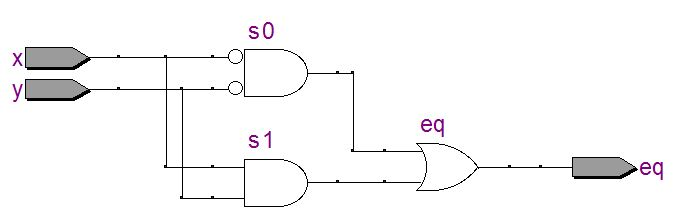
\includegraphics[scale=0.5]{comparator1Bit}
	\caption{1 bit comparator, Listing \ref{vhdl:comparator1Bit}}
	\label{fig:comparator1Bit}
\end{figure}

\begin{explanation}[Listing \ref{vhdl:comparator2Bit}: 2 bit comparator] 
This listing implements the equation \ref{eq:2bitComparator}. Here, we are using two bit input, therefore `std\_logic\_vector' is used at line 8. `1 downto 0' sets the 1 as MSB (most significant bit) and 0 as LSB(least significant bit) i.e. the $a[1]$ and $b[1]$ are the MSB, whereas $a[0]$ and $b[0]$ are the LSB. Since we need to store four signals (lines 16-19), therefore `s' is defined as 4-bit vector in line 14. Rest of the working is same as Listing \ref{vhdl:comparator1Bit}. The implementation of this listing is shown in Fig. \ref{fig:comparator2Bit}. 
\end{explanation}
\lstinputlisting[
language = Vhdl,
caption    = {Comparator 2 Bit},
label      = {vhdl:comparator2Bit}
]{comparator2Bit.vhd}
\begin{figure}[!h]
	\centering
	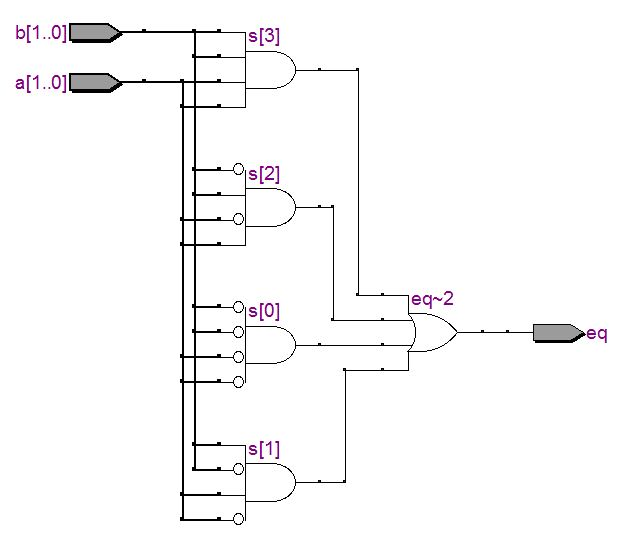
\includegraphics[scale=0.5]{comparator2Bit}
	\caption{2 bit comparator, Listing \ref{vhdl:comparator2Bit}}
	\label{fig:comparator2Bit}
\end{figure}

\subsection{Structural modeling}\label{sec:structureModeling}
In previous section, we designed the 2 bit comparator based on equation \ref{eq:2bitComparator}. Further, we can design the 2 bit comparator using 1-bit comparator as well, with following steps, 
\begin{enumerate}
	\item First compare each bit of 2-bit numbers using 1-bit comparator;  i.e. compare $a[0]$ with $b[0]$ and $a[1]$ with $b[1]$ using 1-bit comparator (as shown in Table \ref{tbl:comparator2Bit}). 
	
	\item If both the values are equal, then set the output `eq' as 1, otherwise set it to zero. 
\end{enumerate}

This method is known as `structural' modeling, where we use the pre-defined designs to create the new designs (instead of implementing the `boolean' expression). This method is quite useful, because most of the large-systems are made up of various small design units. Also, it is easy to create, simulate and check the various small units instead of one large-system. Listing \ref {vhdl:comparator2BitStruct} and \ref{vhdl:comparator2BitStructComponent} are the examples of structural designs, where 1-bit comparator is used to created a 2-bit comparator.  


\begin{explanation}[Listing \ref{vhdl:comparator2BitStruct}]
	In this listing, line 6-11 defines the entity, which has two input ports of 2-bit size and one 1-bit output port. Then two signals are defined (line 14) to store the outputs of two 1-bit comparators, as discussed below.
	
	`$eq\_bit0$' and `$eq\_bit1$' in lines 16 and 18 are the names of the two 1-bit comparator used in this design. We can see these names in the resulted design, which is shown in Fig. \ref{vhdl:comparator2BitStruct}.  
	
	Next, `comparator1bit' in lines 16 and 18 is the name of entity of 1-bit comparator (Listing \ref{vhdl:comparator1Bit}). With this declaration, i.e. comparator1bit, we are calling the design of 1-bit comparator to current design. 
	
	Then, `port map' statements in lines 17 and 19, are assigning the values to the input and output port of 1-bit comparator. For example, in line 17, input ports of 1-bit comparator, i.e. $x$ and $y$, are assigned the values of $a(0)$ and $b(0)$ from this design; and the output $y$ of 1-bit comparator is stored in the signal $s0$. Further, in line 21, if signals $s0$ and $s1$ are 1 then `eq' is set to 1 using `and' gate, otherwise it will be set to 0.
	
	Lastly, `work' in lines 16 and 18, is the compilation library; where all the compiled designs are stored. The statement `work.comparator1bit' indicates to look for the `comparator1bit' entity in `work' library. Final design generated by Quartus software for Listing \ref{vhdl:comparator2BitStruct} is shown in Fig. \ref{fig:comparator2BitStruct}. 
\end{explanation}
\lstinputlisting[
language = Vhdl,
caption    = {Structure modeling using work directory},
label      = {vhdl:comparator2BitStruct}
]{comparator2BitStruct.vhd}
\begin{figure}
	\centering
	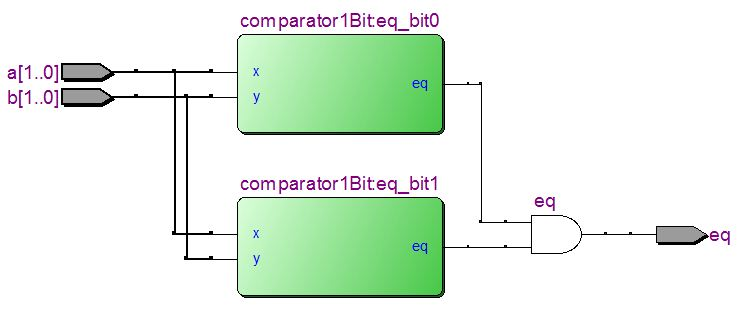
\includegraphics[scale=0.6]{comparator2BitStruct}
	\caption{2 bit comparator, Listing \ref{vhdl:comparator2BitStruct}}
	\label{fig:comparator2BitStruct}
\end{figure}
\begin{explanation}[Fig. \ref{fig:comparator2BitStruct}]
	In this figure, a[1..0] and b[1..0]  are the input bits  whereas `eq' is the output bit. Thick lines after a[1..0] and b[1..0] show that there are more than 1 bits e.g. in this case these lines have two bits. These thick lines are changed to thin lines before going to comparators; which indicates that only 1 bit is sent as input to comparator. 
	
	In `comparator1Bit: eq\_bit0', `comparator1Bit' is the name of the entity defined for 1-bit comparator (Listing \ref{vhdl:comparator1Bit}); whereas the `eq\_bit0' is the name of this entity defined in line 16 of listing \ref{vhdl:comparator2BitStruct}. Lastly outputs of two 1-bit comparator are sent to `and' gate according to line 21 in listing \ref{vhdl:comparator2BitStruct}. 
	
	Hence, from this figure we can see that the 2-bit comparator can be designed by using two 1-bit comparator. 
\end{explanation}



\begin{explanation}[Listing \ref{vhdl:comparator2BitStructComponent}]
	The working of the listing is same as Listing \ref{vhdl:comparator2BitStructComponent}, with some small differences as discussed here. 	In Listing \ref{vhdl:comparator2BitStruct}, work directory is used to find the 1-bit comparator design; whereas in Listing \ref{vhdl:comparator2BitStructComponent}, the 1-bit comparator is explicitly declared as `component' in 2-bit comparator design as shown in line 14-19. Further, in lines 22 and 24 of  Listing \ref{vhdl:comparator2BitStructComponent}, the name of the component i.e. `comparator1Bit' is defined; instead of `work.comparator1Bit' which is used in lines 16 and 18 of Listing \ref{vhdl:comparator2BitStruct}. The final design generated by Quartus software is shown in Fig. \ref{fig:comparator2BitStructComponent} which is exactly same as  Fig. \ref{fig:comparator2BitStruct}.
\end{explanation}

\lstinputlisting[
language = Vhdl,
caption    = {Structure modeling using component declaration},
label      = {vhdl:comparator2BitStructComponent}
]{comparator2BitStructComponent.vhd}
\begin{figure}
	\centering
	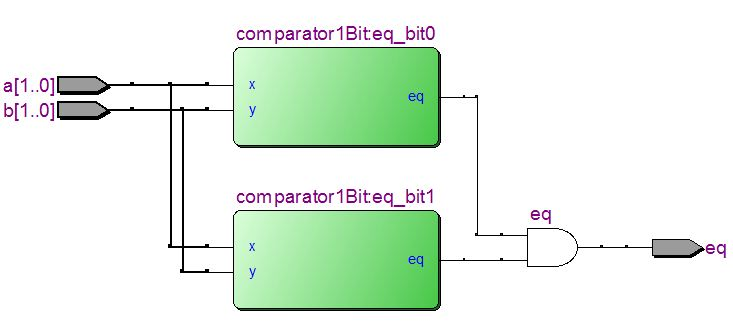
\includegraphics[scale=0.6]{comparator2BitStructComponent}
	\caption{2 bit comparator, Listing \ref{vhdl:comparator2BitStructComponent}}
	\label{fig:comparator2BitStructComponent}
\end{figure}

\begin{itemize}
	\item Note that, multiple architectures can be defined for one entity. For example, in this tutorial, various architectures are created for two bit comparator with different entity names; but these architectures can be saved in single file with one entity name. Then, `configuration' method can be used to select a particular architecture, which may result in complex code.   
	
	\item Throughout the tutorials, we use only single architecture for each entity, therefore `configuration' is not discussed in this tutorial. 
\end{itemize}

\begin{noNumBox}
	Remember that, all the input ports must be connected in `port map' whereas connections with output ports are optional e.g. in line 13, $eq=>s0$ is optional, if we do not need the output `eq' in the current design, then we can skip this declaration. But $x$ and $y$ are the input ports, therefore these connection can not be skipped in port mapping.	 
\end{noNumBox}
\subsection{Behavioral modeling}\label{sec:behaviourModeling}
In behavioral modeling, the `process' keyword is used and all the statements inside the process statement execute sequentially. Various conditional and loop statements can be used inside the process block as shown in Listing \ref{vhdl:comparator2BitProcess}. Further, process blocks are concurrent blocks, i.e. if an architecture body contains multiple process blocks (see Listing \ref{vhdl:comparator2BitProcess2}), then all the process blocks will execute in parallel. 

\begin{explanation}[Listing \ref{vhdl:comparator2BitProcess}: Behavioral modeling]
Entity is declared in line 6-11 which is same as previous codes. In architecture body, the `process' block is declared in line 15, which begins and ends at line 16 and 22 respectively. Therefore all the statements between line 16 to 22 will execute sequentially and Quartus Software will generate the design based on the sequences of the statements.  Any changes in sequences will result in different design.

The `process' keyword takes two argument in line 15 (known as `sensitivity list'), which indicates that the process block will be executed if and only if there are some changes in `a' and `b'. In line 17-21, the `if' statement is declared which sets the value of `eq' to 1 if both the bits are equal (line 17-18), otherwise `eq' will be set to 0 (line 19-20). Fig. \ref{fig:comparator2BitProcess} shows the design generated by the Quartus Software for this listing. `=' in line 17 is one of the condition operators, which are discussed in detail in Chapter \ref{ch:Datatypes}. Unlike python, we can not interchange single ($'$) and double quotation mark ( $''$); single quotation is used for 1-bit (i.e. $'1'$), whereas double quotation is used for more than one bits (i.e. $ ''101''$) e.g. if we use double quotation in line 18, then it will generate error during compilation.    
\end{explanation}
\lstinputlisting[
language = Vhdl,
caption    = {Behavioral modeling},
label      = {vhdl:comparator2BitProcess}
]{comparator2BitProcess.vhd}
\begin{figure}
	\centering
	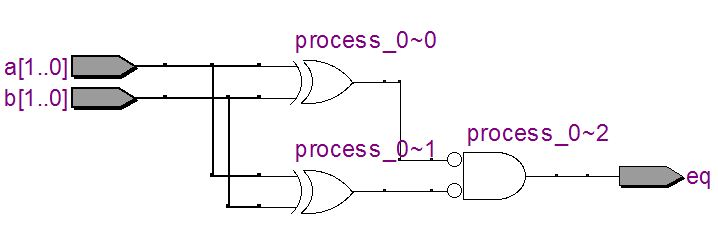
\includegraphics[scale=0.5]{comparator2BitProcess}
	\caption{2 bit comparator, Listing \ref{vhdl:comparator2BitProcess}}
	\label{fig:comparator2BitProcess}
\end{figure}



\subsection{Mixed modeling}
We can mixed all the modeling styles together as shown in Listing \ref{vhdl:comparator2BitProcess2}. Here two process blocks are used in line 16 and 25, which is the behavior modeling style. Then in line 34, dataflow style is used for assigning the value to output variable `eq'.

\begin{explanation}[Listing \ref{vhdl:comparator2BitProcess2}: Mixed modeling]
	Entity is declared in line 6-11, which is same as previous listings. Two process blocks are used here. Process block at line 16 checks whether the LSB of two numbers are equal or not; if equal then signal `s0' is set to 1 otherwise it is set to 0. Similarly, the process block at line 25, sets the value of `s1' based on MSB values. Lastly, line 34 sets the output `eq' to 1 if both `s0' and `s1' are 1, otherwise it is set to 0. The design generated for this listing is shown in Fig. \ref{fig:comparator2BitProcess2}.
\end{explanation}
\lstinputlisting[
language = Vhdl,
caption    = {Behavioral modeling with multiple `process' statements},
label      = {vhdl:comparator2BitProcess2}
]{comparator2BitProcess2.vhd}
\begin{figure}
	\centering
	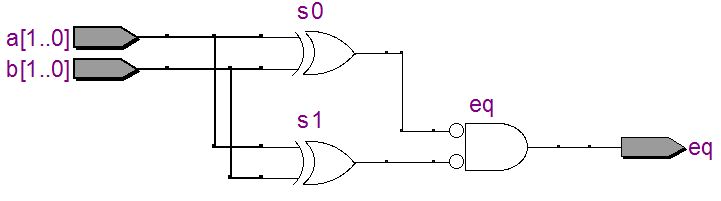
\includegraphics[scale=0.5]{comparator2BitProcess2}
	\caption{2 bit comparator, Listing \ref{vhdl:comparator2BitProcess2}}
	\label{fig:comparator2BitProcess2}
\end{figure}

\section{Packages}
If certain declarations are used frequently, e.g. components and functions etc., then these declaration can store in `packages' as shown in Listing \ref{vhdl:packageEx}. After this, we can import these declaration in the design as shown in Listing \ref{vhdl:comparator2BitPackage}, where the design in Listing \ref{vhdl:comparator2BitStructComponent} is rewritten using packages.

\begin{explanation}[Listing \ref{vhdl:packageEx}: Package declaration]
We define the component `compare1Bit' in Listing \ref{vhdl:comparator2BitStructComponent} for structure modeling. Suppose this component declaration is used at various other designs as well, then it's better to store it in the `package' and call the package in the designs; instead of rewriting the component-declaration in all the designs.

In Listing \ref{vhdl:packageEx}, the package is defined with name `packageEx' (line 6) and inside this package the component `compare1Bit' is defined (line 7-12), which is exactly same as Listing \ref{vhdl:comparator2BitStructComponent}. 
\end{explanation}

\lstinputlisting[
language = Vhdl,
caption    = {Package declaration},
label      = {vhdl:packageEx}
]{packageEx.vhd}

\begin{explanation}[Listing \ref{vhdl:comparator2BitPackage}]
	Next, we need to call the package (defined in Listing \ref{vhdl:packageEx}) to the current design, which can be done as shown in line 6 of Listing \ref{vhdl:comparator2BitPackage}. This line includes the packageEx in the current design. The only difference between Listing \ref{vhdl:comparator2BitPackage} and \ref{vhdl:comparator2BitStructComponent} is the component declaration at line 14-19 in Listing \ref{vhdl:comparator2BitStructComponent}, which is not done in Listing \ref{vhdl:comparator2BitPackage}, as it is imported from package at line 6. The final design generated is shown in Fig. \ref{fig:comparator2BitPackage}, which is exactly same as Fig. \ref{fig:comparator2BitStructComponent}. 
\end{explanation}
\lstinputlisting[
language = Vhdl,
caption    = {Using Packages},
label      = {vhdl:comparator2BitPackage}
]{comparator2BitPackage.vhd}
\begin{figure}
	\centering
	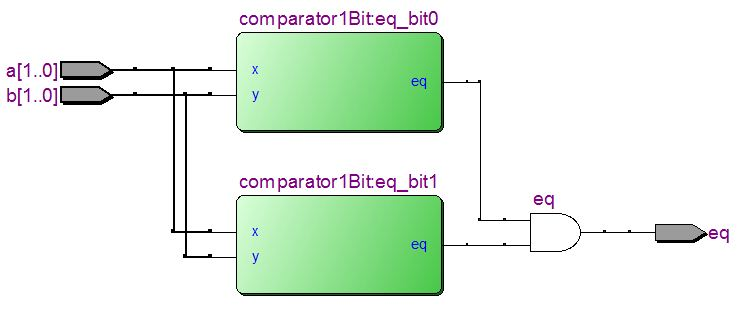
\includegraphics[scale=0.6]{comparator2BitPackage}
	\caption{2 bit comparator, Listing \ref{vhdl:comparator2BitPackage}}
	\label{fig:comparator2BitPackage}
\end{figure}
%\section{Conclusion}
In this tutorial, various features of VHDL designs are discussed briefly. We designed the two bit comparator with four modeling styles i.e. dataflow, structural, behavioral and mixed styles. Also, differences between the generated-designs with these four methods are shown. Lastly, packages are discussed to store the common declaration in the designs. 

\section{Introduction}
VHDL is the hardware description language which is used to model the digital systems. VHDL is quite verbose, which makes it human readable. In this tutorial, following 3 elements of VHDL designs are discussed briefly, which are used for modeling the digital system.. 
\begin{enumerate}
	\item Entity and Architecture
	\item Modeling styles\\
	a. Dataflow modeling\\
	b. Structural modeling\\
	c. Behavioral modeling\\
	d. Mixed modeling
	\item Packages
\end{enumerate}

The 2-bit comparators are implemented using various methods and corresponding designs are illustrated, to show the differences in these methods. All these topics are elaborated in later chapters. Note that, all the features of VHDL can not be synthesized i.e. these features can not be converted into designs. Non-synthesizable features are used to test the design by writing testbenches, which are discussed in Chapter \ref{ch:Testbench}. Rest of the chapters use only those features of VHDL which can be synthesized. All the codes in this tutorial are tested using Modelsim and implemented on FPGA board. Further, the implementation processes, i.e. pin-assignments and downloading the design on FPGA etc, are discussed in Chapter \ref{ch:FirstProject} and \ref{ch:VisualVerification}.

%
%\href{https://www.altera.com/downloads/software/quartus-ii-we/111sp1.html}{`Quartus II 11.1sp1 Web Edition'} and \href{https://www.altera.com/downloads/software/modelsim-starter/111.html}{`ModelSim-Altera Starter'} softwares are used for this tutorial, which are freely available and can be downloaded from the \href{https://www.altera.com/downloads/download-center.html}{Altera website}. All the codes can be \href{http://pythondsp.readthedocs.io/en/latest/pythondsp/toc.html}{downloaded from the website}. First line of each listing in the tutorial, is the name of the python file in the downloaded zip-folder. Also, see Appendix \ref{QuartusModelsim} to compile and synthesize the codes of the tutorial.

\begin{noNumBox}
	Unlike any other electronics designs, if the VHDL design pass the simulation, then it guarantees that it will pass the physical implementation as well. Also, simulation is the only way to verify the large designs and lots of template are shown in Chapter \ref{ch:Testbench}. Some visual verification can also be performed for smaller designs by reducing the clock rate as discussed in Chapter \ref{ch:VisualVerification}.
\end{noNumBox}


\section{Entity and Architecture}
In this section, we discuss `entity declaration' and `architecture body' along with three different ways of modeling i.e. `data flow', 'structural' and `behavioral' modeling. In practice, these three styles are mixed together to model a digital circuit.  

\subsection{Entity declaration}\index{entity}\index{library}
Entity specifies the input-output ports of the design along with optional `generic constants'. The 'generic constants' are discussed in Section \ref{subsec:Generic}. Further, the architecture contains the VHDL codes which describe the functionality of the design, which is converted into hardware by the compiler. Lastly, \textbf{library} contains implementation the commonly used designs. Some of the standard libraries are shown in Section \ref{sec:libPack}. Also, we can create our own libraries using packages which are discussed in Section \ref{sec:ovPackage} and Chapter \ref{ch:Package}. 

In Fig. \ref{fig:andEx}, a simple `and' gate is shown; which is generated by Listing \ref{vhdl:andEx}. Listing \ref{vhdl:andEx} is included to understand the meaning of `entity declaration' and `architecture body'. Also in VHDL, `$--$' is used for comments; please read comments as well to understand the codes.

The entity declaration (lines 6-11) contains all the name of the input and outputs ports as shown in Listing \ref{vhdl:andEx}. Here, the design has two input ports i.e. $x$ and $y$ and one output port i.e. $z$, which are defined inside the `port' block in line 7. Name of the entity `andEx' is defined in line 6. Lastly, we need to import libraries to the listing which contains various functions e.g. library `IEEE' (line 3) contains the package `std\_logic\_1164' (line 4), in which `std\_logic' is defined. `std\_logic' is used in line 8 and 9, to define the 1-bit input and output data-types. Lastly, entity block is closed with `end' keyword in line 11. All these terms, i.e. IEEE library and packages along with data-types, are discussed in detail in Chapter \ref{ch:Datatypes}.  

\begin{figure}
	\centering
	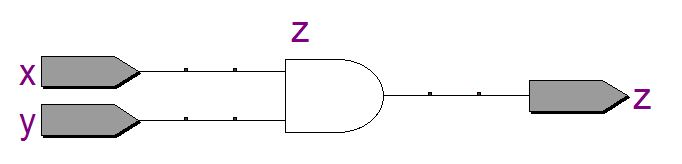
\includegraphics[scale=0.4]{andEx}
	\caption{Circuit generated by Listing \ref{vhdl:andEx}}
	\label{fig:andEx}
\end{figure}

\lstinputlisting[
language = Vhdl,
caption    = {`and' gate example, design: \ref{fig:andEx}},
label      = {vhdl:andEx}
]{andEx.vhd}

\subsection{Architecture body} \index{architecture}
Actual behavior of the design is defined in  the `architecture body'. In Listing \ref{vhdl:andEx}, `and' gate is implemented with `x' and `y' as input, and `z' as output. This behavior is defined in line 15. In line 13, the name of the architecture is defined as `arch' and then name of the entity is given i.e. `andEx'. Complete logic is defined between `begin' and `end' statements i.e. line 14 and 16. Further, we can define intermediate signals of the design (i.e. apart from ports) between line 13-14 as shown in next sections. Next section contains more details about architecture body along with different modeling styles. 

\section{Modeling styles}\index{modeling styles}
In VHDL, the architecture can be defined in four ways as shown in this section. Two bit comparator is designed with different styles; which generates the output `1' if the numbers are equal, otherwise output is set to `0'.   

\subsection{Dataflow modeling}\label{sec:dataflowOverview}\index{modeling styles!dataflow}\index{dataflow modeling}
In this modeling style, the relation between input and outputs are defined using signal assignments. In the other words, we do not define the structure of the design explicitly; we only define the relationships between the signals; and structure is implicitly created during synthesis process. Listing \ref{vhdl:andEx} is the example of dataflow design, where relationship between inputs and output are given in line 15. 

\begin{table}
	\centering
	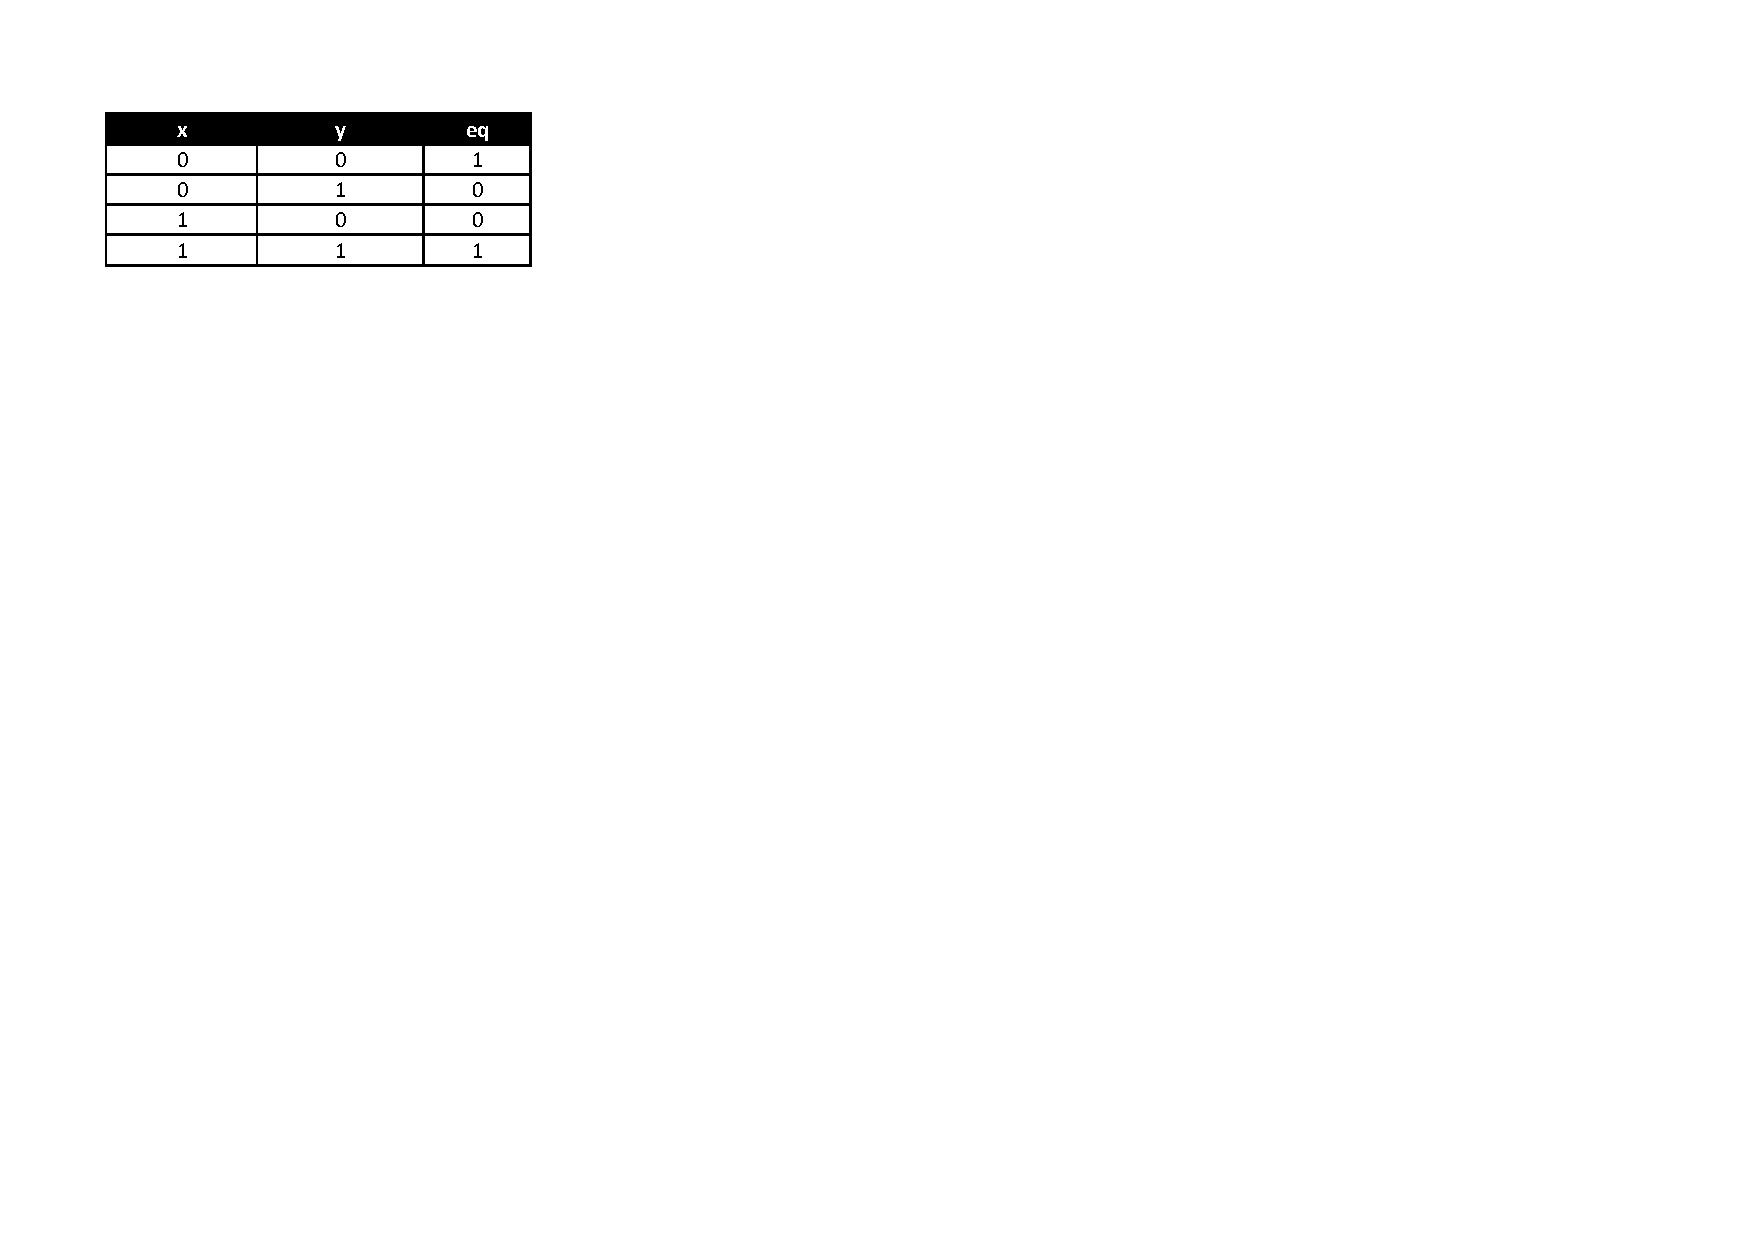
\includegraphics[scale=0.7]{TableComparator1Bit}
	\caption{1 bit comparator, Listing \ref{vhdl:comparator1Bit}}
	\label{tbl:comparator1Bit}
\end{table}

\begin{table}
	\centering
	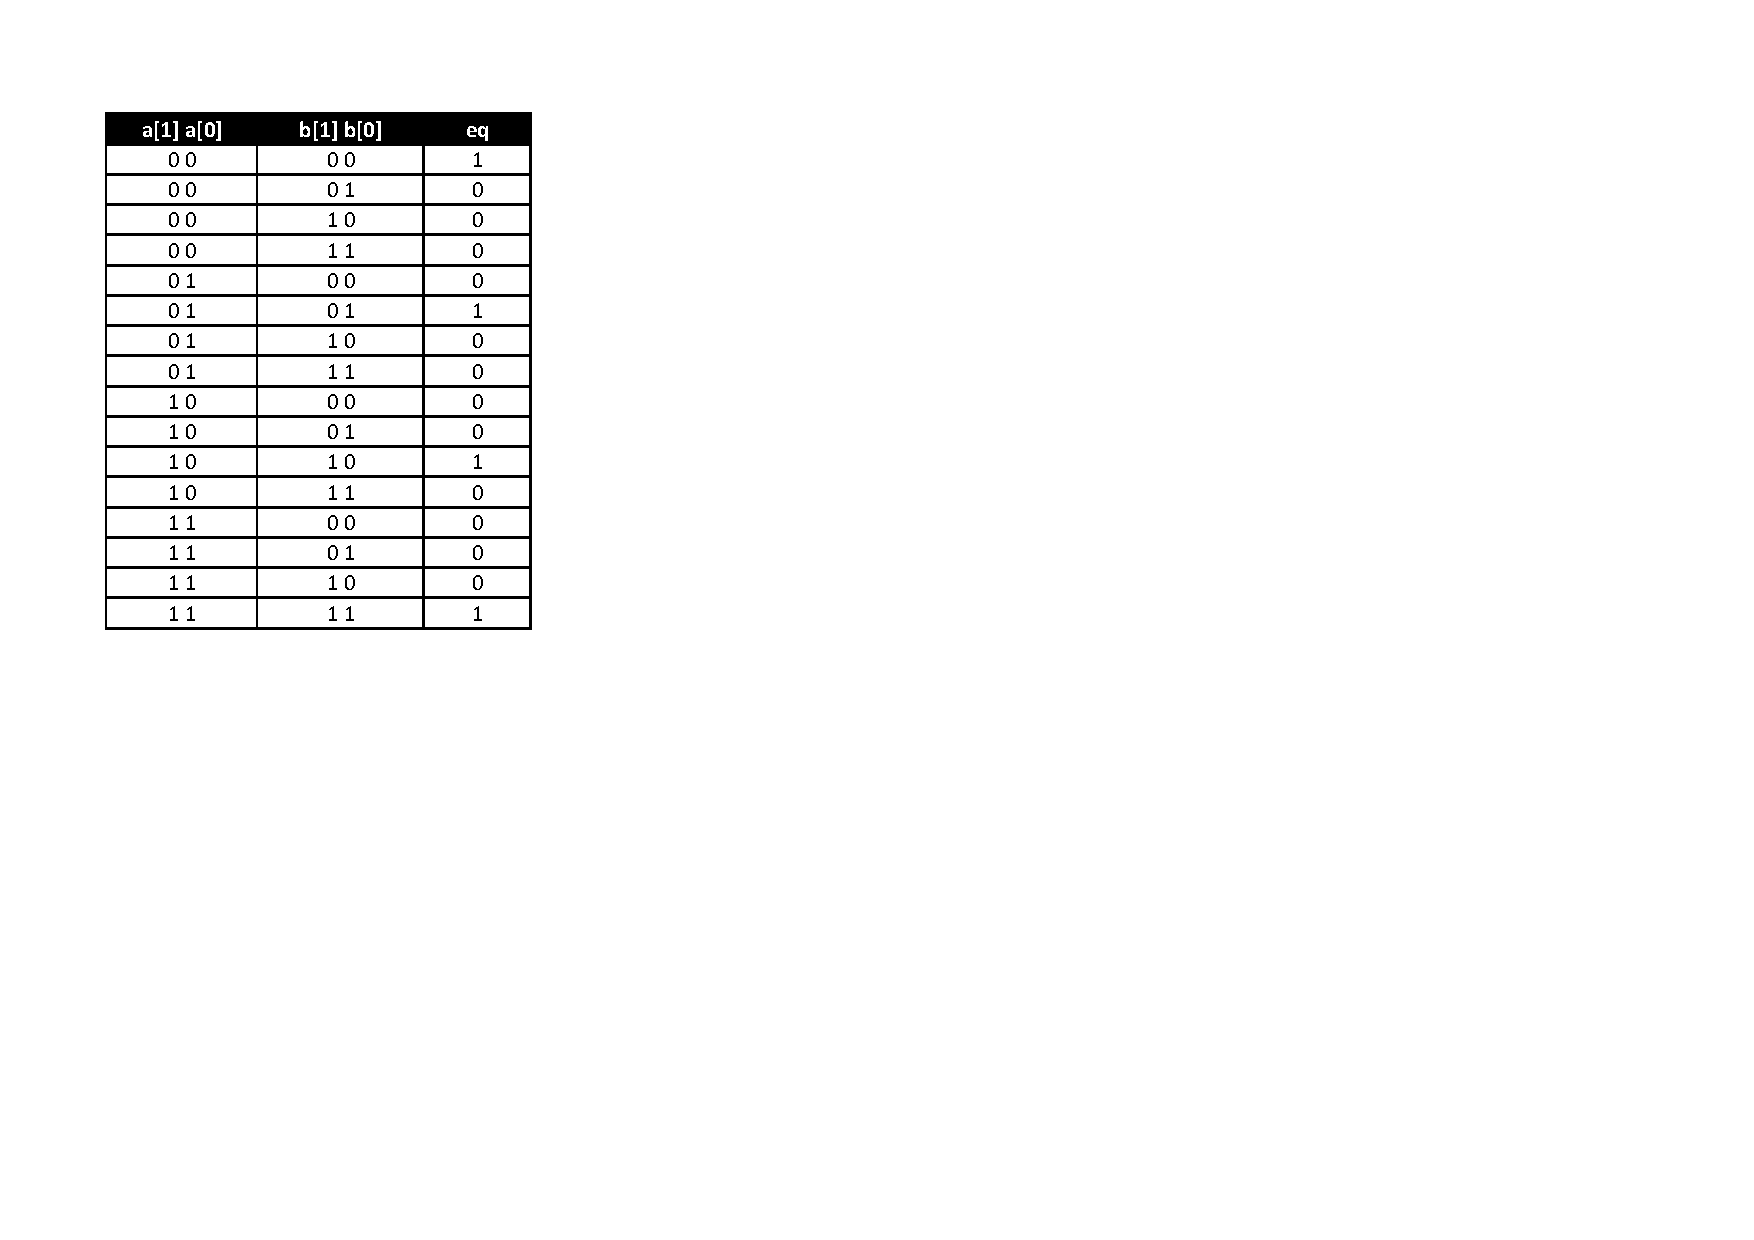
\includegraphics[scale=0.7]{TableComparator2Bit}
	\caption{2 bit comparator, Listing \ref{vhdl:comparator2Bit}}
	\label{tbl:comparator2Bit}
\end{table}

In this section, two more examples of dataflow modeling are shown i.e. `1 bit' and `2 bit' comparators; which are used to demonstrate the differences between various modeling styles in the tutorial. Table \ref{tbl:comparator1Bit} and \ref{tbl:comparator2Bit} show the truth tables of `1 bit' and `2 bit' comparators.  As the name suggests, the comparator compare the two values and sets the output `eq' to 1, when both the input values are equal; otherwise `eq' is set to zero. The corresponding boolean expressions are shown below, 

For 1 bit comparator: 
\begin{equation}
	eq = x' y' + x y
	\label{eq:1bitComparator}
\end{equation} 

For 2 bit comparator: 
\begin{equation}
	eq = a'[1]a'[0]b'[1]b'[0] + a'[1]a[0]b'[1]b[0] + a[1]a'[0]b[1]b'[0] + a[1]a[0]b[1]b[0]
	\label{eq:2bitComparator}
\end{equation} 
Above two expressions are implemented using VHDL in Listing \ref{vhdl:comparator1Bit} and \ref{vhdl:comparator2Bit}, which are explained below.

\begin{explanation}[Listing \ref{vhdl:comparator1Bit}: 1 bit comparator]
	Listing \ref{vhdl:comparator1Bit} implements the 1 bit comparator based on equation \ref{eq:1bitComparator}. Two intermediate signals are defined between `architecture declaration' and `begin' statement (known as declaration section) as shown in line 14. These two signals ($s0$ and $s1$) are defined to store the values of $x'y'$ and $xy$ respectively. Values to these signals are assigned at line 16 and 17. Finally equation \ref{eq:1bitComparator} performs `or' operation on these two signals, which is done at line 19. When we compile this code using `Quartus software', it implements the code into hardware design as shown in Fig. \ref{fig:comparator1Bit}.
	
	The compilation process to generate the design is shown in Appendix \ref{QuartusModelsim}. Also, we can check the input-output relationships of this design using Modelsim, which is also discussed briefly in Appendix \ref{QuartusModelsim}.   
\end{explanation}
\lstinputlisting[
language = Vhdl,
caption    = {Comparator 1 Bit},
label      = {vhdl:comparator1Bit}
]{comparator1Bit.vhd}

\begin{noNumBox}
	Note that, the statements in `dataflow modeling' and `structural modeling' (described in section \ref{sec:structureModeling}) are the concurrent statements, i.e. these statements execute in parallel. In the other words, order of statements do not affect the behavior of the circuit; e.g. if we exchange line 16 and 19 in Listing \ref{vhdl:comparator1Bit}, again we will get the Fig. \ref{fig:comparator1Bit} as implementation. This is discussed in detail in Section \ref{sec:concurrentSeq}. 
	
	On the other hand, statements in `behavior modeling' (described in section \ref{sec:behaviourModeling}) executes sequentially and any changes in the order of statements will change the behavior of circuit. 
\end{noNumBox}

\begin{explanation}[Fig. \ref{fig:comparator1Bit}: 1 bit comparator]
	Fig. \ref{fig:comparator1Bit} is generated by Quartus software according to the VHDL code shown in Listing \ref{vhdl:comparator1Bit}. Here, $s0$ is the `and' gate with inverted inputs $x$ and $y$, which are generated according to line 16 in Listing \ref{vhdl:comparator1Bit}. Similarly,  $s1$ `and' gate is generated according to line 17. Finally output of these two gates are applied to `or' gate (named as `eq') which is defined at line 19 of the Listing \ref{vhdl:comparator1Bit}.   
\end{explanation}
\begin{figure}[!h]
	\centering
	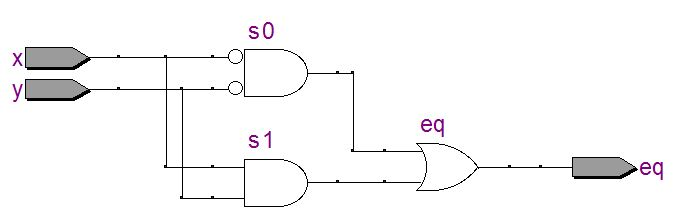
\includegraphics[scale=0.5]{comparator1Bit}
	\caption{1 bit comparator, Listing \ref{vhdl:comparator1Bit}}
	\label{fig:comparator1Bit}
\end{figure}

\begin{explanation}[Listing \ref{vhdl:comparator2Bit}: 2 bit comparator] 
	This listing implements the equation \ref{eq:2bitComparator}. Here, we are using two bit input, therefore `std\_logic\_vector' is used at line 8. `1 downto 0' sets the 1 as MSB (most significant bit) and 0 as LSB(least significant bit) i.e. the $a[1]$ and $b[1]$ are the MSB, whereas $a[0]$ and $b[0]$ are the LSB. Since we need to store four signals (lines 16-19), therefore `s' is defined as 4-bit vector in line 14. Rest of the working is same as Listing \ref{vhdl:comparator1Bit}. The implementation of this listing is shown in Fig. \ref{fig:comparator2Bit}. 
\end{explanation}
\lstinputlisting[
language = Vhdl,
caption    = {Comparator 2 Bit},
label      = {vhdl:comparator2Bit}
]{comparator2Bit.vhd}
\begin{figure}[!h]
	\centering
	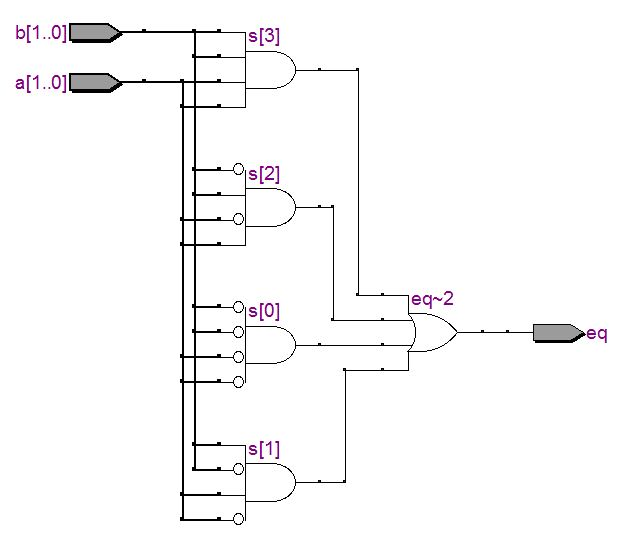
\includegraphics[scale=0.5]{comparator2Bit}
	\caption{2 bit comparator, Listing \ref{vhdl:comparator2Bit}}
	\label{fig:comparator2Bit}
\end{figure}

\subsection{Structural modeling}\label{sec:structureModeling}\index{modeling styles!structural}\index{structural modeling}
In previous section, we designed the 2 bit comparator based on equation \ref{eq:2bitComparator}. Further, we can design the 2 bit comparator using 1-bit comparator as well, with following steps, 
\begin{enumerate}
	\item First compare each bit of 2-bit numbers using 1-bit comparator;  i.e. compare $a[0]$ with $b[0]$ and $a[1]$ with $b[1]$ using 1-bit comparator (as shown in Table \ref{tbl:comparator2Bit}). 
	
	\item If both the values are equal, then set the output `eq' as 1, otherwise set it to zero. 
\end{enumerate}

This method is known as `structural' modeling, where we use the pre-defined designs to create the new designs (instead of implementing the `boolean' expression). This method is quite useful, because most of the large-systems are made up of various small design units. Also, it is easy to create, simulate and check the various small units instead of one large-system. Listing \ref {vhdl:comparator2BitStruct} and \ref{vhdl:comparator2BitStructComponent} are the examples of structural designs, where 1-bit comparator is used to created a 2-bit comparator.  


\begin{explanation}[Listing \ref{vhdl:comparator2BitStruct}]
	In this listing, line 6-11 defines the entity, which has two input ports of 2-bit size and one 1-bit output port. Then two signals are defined (line 14) to store the outputs of two 1-bit comparators, as discussed below.
	
	`$eq\_bit0$' and `$eq\_bit1$' in lines 16 and 18 are the names of the two 1-bit comparator used in this design. We can see these names in the resulted design, which is shown in Fig. \ref{vhdl:comparator2BitStruct}.  
	
	Next, `comparator1bit' in lines 16 and 18 is the name of entity of 1-bit comparator (Listing \ref{vhdl:comparator1Bit}). With this declaration, i.e. comparator1bit, we are calling the design of 1-bit comparator to current design. 
	
	Then, `port map' statements in lines 17 and 19, are assigning the values to the input and output port of 1-bit comparator. For example, in line 17, input ports of 1-bit comparator, i.e. $x$ and $y$, are assigned the values of $a(0)$ and $b(0)$ from this design; and the output $y$ of 1-bit comparator is stored in the signal $s0$. Further, in line 21, if signals $s0$ and $s1$ are 1 then `eq' is set to 1 using `and' gate, otherwise it will be set to 0.
	
	Lastly, `work'\index{work} in lines 16 and 18, is the compilation library; where all the compiled designs are stored. The statement `work.comparator1bit' indicates to look for the `comparator1bit' entity in `work' library. Final design generated by Quartus software for Listing \ref{vhdl:comparator2BitStruct} is shown in Fig. \ref{fig:comparator2BitStruct}. 
\end{explanation}
\lstinputlisting[
language = Vhdl,
caption    = {Structure modeling using work directory},
label      = {vhdl:comparator2BitStruct}
]{comparator2BitStruct.vhd}
\begin{figure}
	\centering
	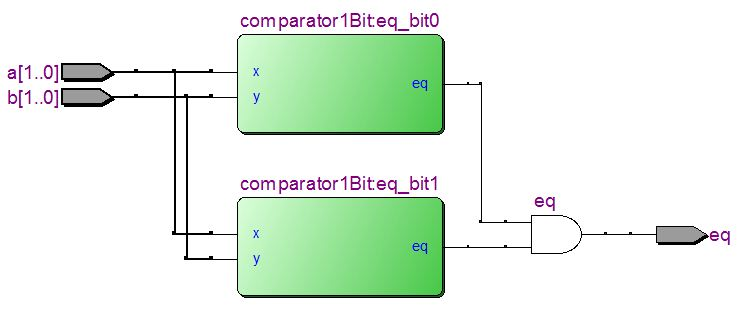
\includegraphics[scale=0.6]{comparator2BitStruct}
	\caption{2 bit comparator, Listing \ref{vhdl:comparator2BitStruct}}
	\label{fig:comparator2BitStruct}
\end{figure}
\begin{explanation}[Fig. \ref{fig:comparator2BitStruct}]
	In this figure, a[1..0] and b[1..0]  are the input bits  whereas `eq' is the output bit. Thick lines after a[1..0] and b[1..0] show that there are more than 1 bits e.g. in this case these lines have two bits. These thick lines are changed to thin lines before going to comparators; which indicates that only 1 bit is sent as input to comparator. 
	
	In `comparator1Bit: eq\_bit0', `comparator1Bit' is the name of the entity defined for 1-bit comparator (Listing \ref{vhdl:comparator1Bit}); whereas the `eq\_bit0' is the name of this entity defined in line 16 of listing \ref{vhdl:comparator2BitStruct}. Lastly outputs of two 1-bit comparator are sent to `and' gate according to line 21 in listing \ref{vhdl:comparator2BitStruct}. 
	
	Hence, from this figure we can see that the 2-bit comparator can be designed by using two 1-bit comparator. 
\end{explanation}



\begin{explanation}[Listing \ref{vhdl:comparator2BitStructComponent}]
	The working of the listing is same as Listing \ref{vhdl:comparator2BitStructComponent}, with some small differences as discussed here. 	In Listing \ref{vhdl:comparator2BitStruct}, work directory is used to find the 1-bit comparator design; whereas in Listing \ref{vhdl:comparator2BitStructComponent}, the 1-bit comparator is explicitly declared as `component' in 2-bit comparator design as shown in line 14-19. Further, in lines 22 and 24 of  Listing \ref{vhdl:comparator2BitStructComponent}, the name of the component i.e. `comparator1Bit' is defined; instead of `work.comparator1Bit' which is used in lines 16 and 18 of Listing \ref{vhdl:comparator2BitStruct}. The final design generated by Quartus software is shown in Fig. \ref{fig:comparator2BitStructComponent} which is exactly same as  Fig. \ref{fig:comparator2BitStruct}.
\end{explanation}

\lstinputlisting[
language = Vhdl,
caption    = {Structure modeling using component declaration},
label      = {vhdl:comparator2BitStructComponent}
]{comparator2BitStructComponent.vhd}
\begin{figure}
	\centering
	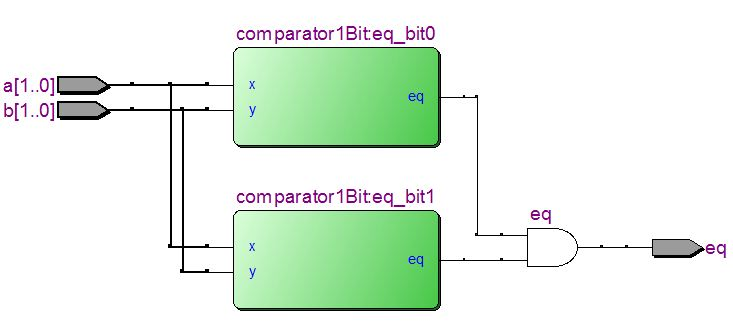
\includegraphics[scale=0.6]{comparator2BitStructComponent}
	\caption{2 bit comparator, Listing \ref{vhdl:comparator2BitStructComponent}}
	\label{fig:comparator2BitStructComponent}
\end{figure}

\begin{itemize}
	\item Note that, multiple architectures can be defined for one entity. For example, in this tutorial, various architectures are created for two bit comparator with different entity names; but these architectures can be saved in single file with one entity name. Then, `configuration' method can be used to select a particular architecture, which may result in complex code.   
	
	\item Throughout the tutorials, we use only single architecture for each entity, therefore `configuration' is not discussed in this tutorial. 
\end{itemize}

\begin{noNumBox}
	Remember that, all the input ports must be connected in `port map' whereas connections with output ports are optional e.g. in line 13, $eq=>s0$ is optional, if we do not need the output `eq' in the current design, then we can skip this declaration. But $x$ and $y$ are the input ports, therefore these connection can not be skipped in port mapping.	 
\end{noNumBox}


\subsection{Behavioral modeling}\label{sec:behaviourModeling}\index{modeling styles!behavioral modeling}\index{behavioral modeling}
In behavioral modeling, the `process' keyword is used and all the statements inside the process statement execute sequentially, and known as `sequential statements'. Various conditional and loop statements can be used inside the process block as shown in Listing \ref{vhdl:comparator2BitProcess}. Further, process blocks are concurrent blocks, i.e. if an architecture body contains multiple process blocks (see Listing \ref{vhdl:comparator2BitProcess2}), then all the process blocks will execute in parallel. 

\begin{explanation}[Listing \ref{vhdl:comparator2BitProcess}: Behavioral modeling]
	Entity is declared in line 6-11 which is same as previous codes. In architecture body, the `process' block is declared in line 15, which begins and ends at line 16 and 22 respectively. Therefore all the statements between line 16 to 22 will execute sequentially and Quartus Software will generate the design based on the sequences of the statements.  Any changes in sequences will result in different design.
	
	The `process' keyword takes two argument in line 15 (known as `sensitivity list'), which indicates that the process block will be executed if and only if there are some changes in `a' and `b'. In line 17-21, the `if' statement is declared which sets the value of `eq' to 1 if both the bits are equal (line 17-18), otherwise `eq' will be set to 0 (line 19-20). Fig. \ref{fig:comparator2BitProcess} shows the design generated by the Quartus Software for this listing. `=' in line 17 is one of the condition operators, which are discussed in detail in Chapter \ref{ch:Datatypes}. Unlike python, we can not interchange single ($'$) and double quotation mark ( $''$); single quotation is used for 1-bit (i.e. $'1'$), whereas double quotation is used for more than one bits (i.e. $ ''101''$) e.g. if we use double quotation in line 18, then it will generate error during compilation.    
\end{explanation}
\lstinputlisting[
language = Vhdl,
caption    = {Behavioral modeling},
label      = {vhdl:comparator2BitProcess}
]{comparator2BitProcess.vhd}
\begin{figure}
	\centering
	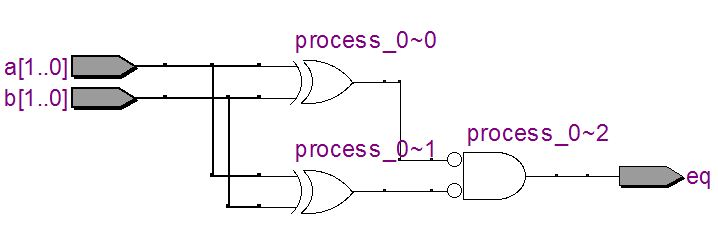
\includegraphics[scale=0.5]{comparator2BitProcess}
	\caption{2 bit comparator, Listing \ref{vhdl:comparator2BitProcess}}
	\label{fig:comparator2BitProcess}
\end{figure}



\subsection{Mixed modeling}\index{modeling styles!mixed modeling}\index{mixed modeling}
We can mixed all the modeling styles together as shown in Listing \ref{vhdl:comparator2BitProcess2}. Here two process blocks are used in line 16 and 25, which is the behavior modeling style. Then in line 34, dataflow style is used for assigning the value to output variable `eq'.

\begin{explanation}[Listing \ref{vhdl:comparator2BitProcess2}: Mixed modeling]
	Entity is declared in line 6-11, which is same as previous listings. Two process blocks are used here. Process block at line 16 checks whether the LSB of two numbers are equal or not; if equal then signal `s0' is set to 1 otherwise it is set to 0. Similarly, the process block at line 25, sets the value of `s1' based on MSB values. Lastly, line 34 sets the output `eq' to 1 if both `s0' and `s1' are 1, otherwise it is set to 0. The design generated for this listing is shown in Fig. \ref{fig:comparator2BitProcess2}.
\end{explanation}
\lstinputlisting[
language = Vhdl,
caption    = {Behavioral modeling with multiple `process' statements},
label      = {vhdl:comparator2BitProcess2}
]{comparator2BitProcess2.vhd}
\begin{figure}
	\centering
	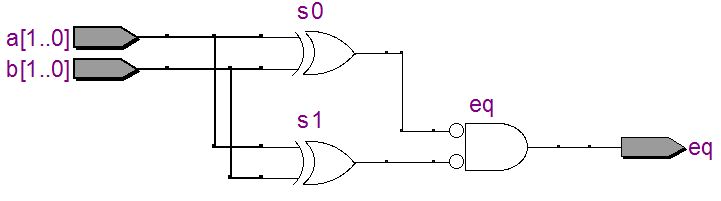
\includegraphics[scale=0.5]{comparator2BitProcess2}
	\caption{2 bit comparator, Listing \ref{vhdl:comparator2BitProcess2}}
	\label{fig:comparator2BitProcess2}
\end{figure}

\section{Packages}\label{sec:ovPackage}\index{packages}
If certain declarations are used frequently, e.g. components and functions etc., then these declaration can store in `packages' as shown in Listing \ref{vhdl:packageEx}. After this, we can import these declaration in the design as shown in Listing \ref{vhdl:comparator2BitPackage}, where the design in Listing \ref{vhdl:comparator2BitStructComponent} is rewritten using packages.

\begin{explanation}[Listing \ref{vhdl:packageEx}: Package declaration]
	We define the component `compare1Bit' in Listing \ref{vhdl:comparator2BitStructComponent} for structure modeling. Suppose this component declaration is used at various other designs as well, then it's better to store it in the `package' and call the package in the designs; instead of rewriting the component-declaration in all the designs.
	
	In Listing \ref{vhdl:packageEx}, the package is defined with name `packageEx' (line 6) and inside this package the component `compare1Bit' is defined (line 7-12), which is exactly same as Listing \ref{vhdl:comparator2BitStructComponent}. 
\end{explanation}

\lstinputlisting[
language = Vhdl,
caption    = {Package declaration},
label      = {vhdl:packageEx}
]{packageEx.vhd}

\begin{explanation}[Listing \ref{vhdl:comparator2BitPackage}]
	Next, we need to call the package (defined in Listing \ref{vhdl:packageEx}) to the current design, which can be done as shown in line 6 of Listing \ref{vhdl:comparator2BitPackage}. This line includes the packageEx in the current design. The only difference between Listing \ref{vhdl:comparator2BitPackage} and \ref{vhdl:comparator2BitStructComponent} is the component declaration at line 14-19 in Listing \ref{vhdl:comparator2BitStructComponent}, which is not done in Listing \ref{vhdl:comparator2BitPackage}, as it is imported from package at line 6. The final design generated is shown in Fig. \ref{fig:comparator2BitPackage}, which is exactly same as Fig. \ref{fig:comparator2BitStructComponent}. 
\end{explanation}
\lstinputlisting[
language = Vhdl,
caption    = {Using Packages},
label      = {vhdl:comparator2BitPackage}
]{comparator2BitPackage.vhd}
\begin{figure}
	\centering
	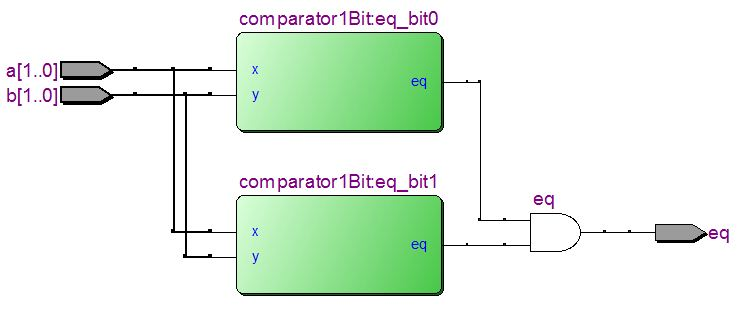
\includegraphics[scale=0.6]{comparator2BitPackage}
	\caption{2 bit comparator, Listing \ref{vhdl:comparator2BitPackage}}
	\label{fig:comparator2BitPackage}
\end{figure}


\section{Conclusion}
In this tutorial, various features of VHDL designs are discussed briefly. We designed the two bit comparator with four modeling styles i.e. dataflow, structural, behavioral and mixed styles. Also, differences between the generated-designs with these four methods are shown. Lastly, packages are discussed to store the common declaration in the designs. 